%% This document gives an example on how to use the ntnumasterthesis
%% LaTeX document class.

%% Use short name MACS, MIS, CIMET, MTDMT, MIXD or MIS  
%% Language english or norsk
%% b5paper with oneside or twoside, you can set A4 if you want but you submit in b5

%% If you want print with the heading material on a4 paper you can use this format
%% \documentclass[MACS,english,a4paper,oneside,12pt]{ntnuthesis/ntnuthesis}

%% with the change to using DAIM we have a new option. include DAIM after english below removes the front page material so that you can then submit in the DAIM system. If you are wanting the front material remove DAIM and make sure you fill in the DaimData.tex file.
\documentclass[MIXD,english]{ntnuthesis/ntnuthesis}

\usepackage[T1]{fontenc}
\usepackage[utf8]{inputenc}     % For utf8 encoded .tex files allows norwegian characters in the files. This can be dangerous if you change to a differnt editor.
%\usepackage[pdftex]{graphicx, hyperref}   % For cross references in pdf
\usepackage{graphicx}
\usepackage{hyperref}   % For cross references in pdf


\usepackage{color}              % For colouring text 
\hypersetup{colorlinks=true,     
		linkcolor=blue,          % color of internal links (change box color with linkbordercolor)
    citecolor=blue,        % color of links to bibliography
    filecolor=blue,      % color of file links
    urlcolor=blue           % color of external links
		}
\usepackage{csvsimple}  % for simple table reading and display
\usepackage{url}
\usepackage{booktabs}
\usepackage{gnuplottex} %miktex option if using miktex on windows
\usepackage{rotating}
\usepackage{float}


\definecolor{darkgreen}{rgb}{0,0.5,0}
\definecolor{darkred}{rgb}{0.5,0.0,0}

\lstset{        basicstyle=\ttfamily,
                keywordstyle=\color{blue}\ttfamily,
                stringstyle=\color{darkred}\ttfamily,
                commentstyle=\color{darkgreen}\ttfamily,
}


%Typesetting of C++ but not always stable in titles etc...
\newcommand{\CPP}[0]{{C\nolinebreak[4]\hspace{-.1em}\raisebox{.1ex}{\small\bf +\hspace{-.1em}+\ }}}

%\usepackage[table]{xcolor}% http://ctan.org/pkg/xcolor
%\usepackage[nomessages]{fp}
%\newlength{\maxbarlen}


\newcommand\databar[3][gray!20]{%
  \FPeval\result{round(#3/#2:4)}%
  \rlap{\textcolor{#1}{\hspace*{\dimexpr-\tabcolsep+.5\arrayrulewidth}%
        \rule[-.05\ht\strutbox]{\result\maxbarlen}{.95\ht\strutbox}}}%
  \makebox[\dimexpr\maxbarlen-2\tabcolsep+\arrayrulewidth][r]{#3}}



\newcommand{\com}[1]{{\color{red}#1}} % supervisor comment
%\renewcommand{\com}[1]{} %remove starting % to remove supervisor comments
% This will appear in text \com{Lecuters comment} and be visible unless you uncomment
% the renewcommand line.

\newcommand{\todo}[1]{{\color{green}#1}} % items to do
%\renewcommand{\todo}[1]{} %remove starting % to remove items to do

\newcommand{\n}[1]{{\color{blue}#1}} % other comment
%\renewcommand{\n}[1]{} %remove starting % to remove notes

\newcommand{\dn}[1]{} % add the d to a note to say that you have finished with it.





% Set to true ONLY if using Harvard citation style
\newboolean{HarvardCitations}
\setboolean{HarvardCitations}{true} % false for computer science, true for interaction design and harvard style


\ifthenelse{\boolean{HarvardCitations}}{%
	\usepackage{natbib} % for Harvard names as citations.
}{%
	\usepackage[numbers]{natbib} % for Vancover numbers in bibliography
}

\newcommand{\q}[1]{\leavevmode\marginpar{\small\em #1}}
\renewcommand{\q}[1]{}


\begin{document}

% for students submitting in the DAIM system this information will not be used.
% their is an option for DAIM submission which removes this information and checks it is B5.
% Removing the DAIM option on the document type will use this material.

\setthesistitle{User-centred Chatbot Personalities: a stable pattern for a more effective design processes of conversational interfaces}
\setthesisshorttitle{User-centred chatbot personalities} % a short version for the page headers if your normal title is too long to fit
\setthesisauthor{Tuva Lunde Smestad}
\setthesissupervisor{Frode Volden}
\setthesissupervisorA{Anders-Petter Andersson}  % if you have a second supervisor add it like this
%\setthesissupervisorB{Prof. Smart Guy}  % if you have a second supervisor add it like this


\nmtkeywords{Personality, Chatbot, Conversational Interfaces, Thesis, User Centred Design, User Experience, Personality, Character Development}
%\nmtdesc{This is the short description of a masters thesis}


\setthesisdate{01-06-2018}
\setthesisyear{2018}



%for CIMET theses you need to see all of these as well

%\setthesiscampus{Gj\o{}vik}
%\setthesisHostInstitution{\NTNU}
%\setthesisHostInstitution{University of Eastern Finland}
%\setthesisHostInstitution{Universit\'e Jean Monnet Saint-Etienne}

%\setthesisjuryA{} %jury names
%\setthesisjuryB{} %jury names
%\setthesisjuryC{} %jury names
%\setthesisjuryD{} %jury names


 % this is the file which contains all the details about your thesis
\makefrontpages % make the frontpages
%this is the intro to the thesis
%\thesistitlepage % make the ordinary titlepage
\hypersetup{pageanchor=false}
%\include{summary}

\chapter*{Preface}
This master thesis is the final part of my Master in Interaction Design degree at the department of Design at the Norwegian University of Science and Technology (NTNU). The project planning and preliminary studies/literature review was conducted during the autumn of 2017. The work presented in this thesis was conducted and written during the spring of 2018 and the workload corresponds to 30 ECTS.

Throughout my work as an interaction designer I was challenged with building my first chatbot and was surprised to find that much work is still to be done regarding the user experience of chatbots. Most of the frameworks acts more like "do's" and "dont's" rather than based on research. And a lot of these guidelines are based on assumptions, or small case studies that do not necessarily extends to the larger application of conversational agents. Not wanting chatbots to be abandoned early by users because the implementation of these systems are far behind the technological development, I set out with this thesis to try and prove at least one assumption: does personality improve the user experience of chatbots?

I aim with this master thesis to add to the field of human-computer and human-robot interaction by providing evidence to explain how personality impacts the user experience of machines that can converse. In addition to this I'm also providing other designers and developers, interested in conversational interfaces, with a framework to build synthetic personalities for chatbot agents.

This thesis is for anyone who wishes to design their own chatbot with a basis in personality, and those who like me are eager to determine how we can improve the user experience of conversational interfaces.

\vspace{5mm}

%\begin{center}
%\thesiscampus, 
\thesisdate \\[1pc]
\\[1pc]
%\thesisauthor
%\end{center}

\chapter*{Acknowledgment}
I would like to thank the following persons for their great help during the course of this thesis project:

\vspace{5mm}

My partner Christopher Solem for providing emotional support, extraordinary listening skills, helpful commentary and for proof reading not only my thesis, but the literature review and project planning report. I would not have survived my masters degree without you.

\vspace{5mm}

Mom and dad for their long standing support, both emotional and material, and for lending me your car so I could get around to all who participated in my experiment.

\vspace{5mm}

The participants for taking time out of their busy schedule to help me with my thesis project.

\vspace{5mm}

My supervisor Frode Volden, for keeping my research aim on track, reminding me to not forget about the overall aim and not become too concerned about the design and building of the chatbot prototype. I am grateful for all your help and your sound knowledge in SPSS, which I would not have made it without!

\vspace{5mm}

My co-supervisor Anders-Petter Andersson for providing challenging questions that made me stop to reassess and question my choices throughout the process. Pointing me in the direction of valuable resources and articles, designs and research to help me get a thorough understanding of the field I now have explored.

\begin{flushright}
T.L.S.\\[1pc]
\end{flushright}

\include{Abstract}



\tableofcontents

\hypersetup{pageanchor=true}

% Comment with a percent to remove figures or tables:
\listoffigures
\listoftables
\chapter*{Acronyms}

\begin{itemize}[label={}]
    \item \textbf{UCD} \hspace{2mm} User Centred Design
    \item \textbf{UX} \hspace{2mm} User Experience
    \item \textbf{CUI} \hspace{2mm} Conversational User Interface
    \item \textbf{VUI} \hspace{2mm} Voice User Interface
    \item \textbf{NUI} \hspace{2mm} Natural User Interface
    \item \textbf{AI} \hspace{2mm} Artificial Intelligence
    \item \textbf{NLP} \hspace{2mm} Natural Language Processing
    \item \textbf{API} \hspace{2mm} Application Programming Interface
    \item \textbf{UI} \hspace{2mm} User Interface
    \item \textbf{CA} \hspace{2mm} Conversational Agent
    \item \textbf{VA} \hspace{2mm} Virtual Agent
    \item \textbf{ECA} \hspace{2mm} Embodied Conversational Agent
    \item \textbf{SDS} \hspace{2mm} Spoken Dialogue System
    \item \textbf{PM} \hspace{2mm} Project Manager
    \item \textbf{OCEAN} \hspace{2mm} Openness, Conscientiousness, Extroversion, Agreeableness, Neuroticism
    \item \textbf{HEXACO} \hspace{2mm} Honesty-humility, Emotionality, eXtraversion, Agreeableness, Conscientiousness, Openness
    \item \textbf{TOV} \hspace{2mm} Tone of Voice
    \item \textbf{PQ} \hspace{2mm} Pragmatic Quality
    \item \textbf{HQ-I} \hspace{2mm} Hedonic Quality - Identity
    \item \textbf{HQ-S}\hspace{2mm}  Hedonic Quality - Stimulation
    \item \textbf{ATT} \hspace{2mm} Attractiveness
    \item \textbf{IoT} \hspace{2mm} Internet of Things
\end{itemize}


\chapter{Introduction}
\label{chap:introduction}
\q{What is the purpose of this document?}
The purpose of the current document is to provide an example of using the thesis template and a description on how to use \LaTeX. There are instructions that relate specifically to the template, and some which are generally useful for \LaTeX. 

\q{Where is the structure defined } 
The detailed typographical rules have been implemented in the
\texttt{ntnuthesis} \LaTeX\ document class, in the file 

This was updated by Simon McCallum.
The package has changed names and version number it is now called
\texttt{ntnuthesis}
v\ntnuthesisversion\ as of \ntnuthesisdate.

\q{what is a thesis about}
For many of you, this Master's thesis will be the most advanced academic document you ever write.  It needs to demonstrate both academic ability and clear thinking. You Master's should show that you are ready to lead other people, reflect more deeply, and have a professional attitude to your work and environment. 

\q{who cares}
When writing the thesis it is important to know who you are writing for. The target audience for this document is in layers:
\begin{enumerate}
    \item The marking committee
    \item Your supervisor
    \item Other students at the same level 
    \item Professionals \& Academics
    \item The general public.
\end{enumerate}

\section{Problem Description}
The chatbots of 2017 have not truly improved since the first chatbot ELIZA back in 1966. While the programming behind conversational interfaces are fast improving, making use of Artificial Intelligence (AI) and Natural Language Processing (NLP), a chatbot is still a form of weak-AI in which makes use of stimulus-response approach. Human interaction and conversation consists of a lot more than predicting user intentions, analyse keywords to define meaning, and then respond from a predefined set of responses. Therefore, no matter how accurate the chatbot is in predicting what humans actually mean, and how well it performs its tasks, they are not perceived as intelligent conversational entities. Predictions and recent research find chatbots to be a big part of an AI powered future, but recent reviews of chatbots have found them to be unintelligent and non-conversational (Stokke, 2017, Orf, 2017, Piltch, 2017, Vincent, 2017, Boutin, 2017). Piltch (2017) states that we should not be carried away by the positive outlook researchers presents in regards to the possibilities of advances in AI technology for chatbot technology, as the reality is that most chatbots are falling flat. Despite cautions and recent negative reviews, Forrester (2017) found that 56 \% of companies have implemented or are planning to implement a chatbot as part of the services they provide in the near future. JuniperResearch (2017) released a report in which they have found that chatbots will save companies \textdollar 8 billion in costs by 2022. Therefore, as the trends predict many benefits for companies implementing chatbots, are we forcing users to adopt technology which they find frustrating and useless? If the reviews find chatbot interactions as unintelligent, pointless, and not more effective than conducting a Google search or contacting a human customer service agent, what effects might this have on the user experience?

\section{Justification, Motivation and Benefits}
Ever since ELIZA, the goal of chatbot systems have been to pass the Turing Test, and convince humans that they are conversing with a human, not a machine \citep{McTear2016b}. However, available chatbots does not appear to possess human conversational skills, rather they perform as a machine by responding to user commands. This shows that although a chatbot is more flexible in regards to it being able to understand vast variations of the same command, it still functions as a command-based system. To be perceived as conversational agents, chatbots needs to be able to do a lot more than input-output. Therefore, understanding why chatbots are failing to be conversational and what we can do to allow users to perceive them as more than a computer, can have a great impact on improving the user experience. To understand how we can design chatbots that are perceived as more conversational, means that we must take into account many other factors of human interaction beyond only language understanding. Humans have bodies, feelings, emotions, different personalities and behaviours that all influence how we communicate, behave, and interact. Humans are extremely skilled social actors, and in order to design chatbots that too are skilled social actors we must understand the social cues that make up human interaction, and the personalities that drives them. 

This master thesis project will explore how we can build chatbots that offer a better user experience and are perceived as more conversational through focusing on the design of chatbot personalities. The thesis will understand how thinking about the chatbot as a character with a mind of its own, can benefit the design process and result in more conversational and improved user experience. In addition to this, chatbots are extensions of services provided by companies, therefore it is also important to design personalities that reflects the brand it represents. Through this topic the researcher hopes to add to the understanding of how designers can create better chatbot interfaces, and offer a framework to inform how designing chatbot personalities can benefit the design process as a whole. As trends show that companies are rapidly implementing chatbots as part of their services, consumers should not be forced to adopt solutions that does not improve the effectiveness, efficiency or satisfaction. This investigation would also benefit companies, as this knowledge can help ensure improved services for their customers, and consistent communication in its tone of voice through the chatbot.

\section{Research Questions}
The research questions and sub-questions to be addressed in the master thesis project are:

\begin{enumerate}
    \item How can we design chatbot personalities to guide the design process of a chatbot interface and create a better user experience?
    \subitem a) Which elements must be considered to inform a chatbot personality?
    \subitem b) What components needs to be in place for a chatbot personality to meet user needs and expectations?
    \item How can personality be used as a design variable to allow users to perceive chatbots as more than a computer?
        \subitem a) How can designers use personality to improve the conversational design of chatbots?
        \subitem b) How will the personality affect the user experience?
        \end{enumerate}

\section{Planned Contributions}
The results from exploring techniques to design user-centred chatbot personalities will be presented to define a UX framework that designers can use to build user centred chatbot personalities. This master thesis will produce a framework that entails different methods and techniques that designers can use to design a chatbot persona that meets user needs and is consistent with the brand's tone of voice. This framework will form a foundation to guide the design process of chatbots, towards improved user experience. This framework will inform what elements that needs to be considered to inform the type of personality that is appropriate, and which methods that could help design the personality to be in line with users' needs as well as the brand it represents. This framework will also inform how the chatbot personality can be used to guide and inform other aspects of the design of chatbots such as the conversation design. The framework will include methods to not only design, but evaluate design decisions in relation to the user experience, show how companies can extend and add value to their brands by providing a chatbot experience that is consistent with the brand's tone of voice. % includes latex files from the same directory
\chapter{Theory, Background, Existing Literature}
\label{chap:background}

%explain user experience as well - operationalise it - how it will be evaluated. As well as UCD and more on the role of the chatbot

To understand the scope of research related to the interaction between chatbots and humans, and to understand what important factors to consider to design chatbot personalities, the researcher conducted a literature review as part of the course \textit{IMT4215 Specialisation Project}. This review investigated the scope of research as it related to how humans perceive computers that talk, by looking at research related to the effect anthropomorphism, humanness, and personality have on the user experience of conversational interfaces. The review was concerned with theories in human-computer interaction research, while also exploring human-robot interaction, and theories within human factors and psychology. Through this review the researcher found that emotional intelligence, anthropomorphism, humanness, politeness, human etiquette, humour and gender are important variables to consider when designing a CA, as these are important to how users perceive and experience a CA. In addition, the review also found that researchers \citep{callejas2011,Xiao2005,McTear2016a} believe that personality can be used as a stable pattern to form the behaviour and characteristics of a CA and manage how humans perceive the system. Findings from this review will be summarised and discussed in this chapter in addition to the theory and background regarding chatbots, and how personality theory and insights from branding can inform the design of chatbot personalities.

\vspace{5mm} %5mm vertical space

\section{Chatbots and Conversational Agents}

Chatbots are considered to be a form of "weak AI" \citep{DeAngeli2008}, this means that they do not exceed human intelligence and are often used to complete tasks and for analysing and processing information. Chatbots follow scripted rules, and respond from a set of stored, pre-defined responses, with the goal of simulating human language and conversation. This approach, called a "stimulus-response approach" \citep[: 57]{McTear2016b}, was first realised with the ELIZA chatbot back in 1966. ELIZA was a conversational agent, written by \cite{Weizenbaum1966}, that played the role as a Rogerian psychotherapist very convincingly. The stimulus-response approach functioned by ELIZA matching the user input against a large set of stored patterns, which informed its response output. This means that ELIZA makes a prediction in regards to which of its responses matches to the user's query. This approach proved to be very successful for ELIZA's role as a psychotherapist, and made it appear that she was convincingly conversing with users. The same approach is still used today, and there are two different models: retrieval-based models and generative models \citep{Kothari2016}. The first model uses predefined responses, while the generative model can put together new responses based on users' input. The second model is of course much more difficult to implement, while the first model provides control of which responses the chatbot gives and is much quicker and easier to build and implement. Most of the chatbots we see today that are provided by brands, are based on the retrieval-based models. While being more in control of the output of the chatbots in the retrieval-based model, the downside is that they often appear as less intelligent and are prone to errors if they fail to recognise the correct user intention. ELIZA was successful when she conversed with users, because her role as a psychotherapist allowed her to act like she knew nothing of the world \citep{Weizenbaum1966}. The way in which ELIZA conversed, "tell me more about x", appeared familiar and consistent to how therapy sessions are usually run, and therefore supported users' mental model and expectations when conversing with a therapist. ELIZA inspired future generations of chatbots to simulate human natural language, and ultimately beat Alan \cite{Turing1950} "Imitation Game": to convince humans that they are conversing with a human, not a machine. Therefore, the history and development of chatbots have always had this goal in mind. Today we see chatbots in education, customer service, e-commerce, as virtual assistants or plainly for entertainment as recent advances in machine learning allows for more advanced AI and NLP capabilities for chatbots.

Michael \cite{Mauldin1994} coined the term Chatterbots, which today is known as chatbots, to describe the robots that humans could chat with. Chatbots are conversational agents within the broader term conversational user interfaces (CUI). There are many terms used to describe CUIs such as natural user interfaces (NUI), voice user interfaces (VUI), no user interface or invisible user interface.  CUI and NUI are often used interchangeably, however a NUI often allow for other natural inputs beyond conversation such as touch and gestures. While chatbots refers to CUIs in which users interact with through a chat interface, a VUI only interacts through voice input and output (e.g. Apple's Siri) \citep{Pearl2017}. Other types of conversational interfaces or conversational agents includes spoken dialogue systems (SDS), embodied conversational agents (ECAs) and social robots \citep{McTear2016b}. ECAs make use of facial expressions, animated bodies, and other gestures as well as speech to engage with users. An ECA is therefore a form of a chatbot that make use of more elements than speech to add to the conversation. With the emergence of speech recognition technology and mobile devices, it is common that chatbots also support voice input-output to allow for a more accessible interface.

Conversational agents therefore come in a variety of different forms and purposes, but they all use conversation to interact with humans. Chatbots were originally designed to be conversational partners, rather than a system to help users perform tasks \citep{McTear2016a}. Today this definition has changed, as the trends show an increasing rise in the popularity of chatbots as virtual assistants (VA) on the web. Companies are rapidly implementing chatbots as an extension of the services they provide to their customers, moving beyond its role as a conversational partner. As stated earlier, a report published by \cite{forrester2017} found that 57 \% of companies either use or plan to implement a chatbot in the near future. The conversational element is used to offer a natural way to interact with brands to retrieve information, service support, product purchasing, or other uses. This trend can be explained by the commercial access to APIs which provides easy access to AI and NLP. In addition to this there is a rise in messaging platforms that supports the hosting of chatbots such as Facebook Messenger, Slack, and Skype among others. Humans have also been introduced to CAs more in their everyday life, as most smartphones offer voice assistants to help manage tasks (e.g. Apple's Siri, Google Assistant, Microsoft Cortana).

This rapid trend has had its downside, as too many of these chatbots perform poorly, and their conversational skills do not meet user expectations \citep{stokke2017,boutin2017}. Recently the Norwegian website DinSide.no reviewed Norwegian customer service chatbots implemented in 2017 and the headline reads: "So Stupid Are the Norwegian Robots" \cite{stokke2017}. The article concludes that Google is more efficient in answering your questions, and more accurate, than the customer service chatbots. The reason for this conclusion is that the user needs to adapt its language for the chatbot to understand their query, which can be a time-consuming process, and the conversational element is missing. Apparently, access to AI and NLP is not what makes or breaks a chatbot, and designers must explore other approaches and techniques to design better conversational interfaces.

\vspace{5mm} %5mm vertical space

\section{Personality to Dictate Human Perception}
    \label{humanperception}

Through the literature review, the researcher investigated how humans perceive conversational agents and which factors that can be used to influence human perception. The findings suggests that personality is an important factor in relation to alter and dictate the way in which humans perceive CAs. The following sections will provide a summary of the most important findings from the literature review and why personality is so important to the design of CAs.

\vspace{2,5mm}

\subsection{Emotions and personality}
    \label{emotionspersonality}
Emotional intelligence is an important part of how humans perceive themselves as intelligent beings. In order to assess artificial intelligence critics have always used emotional intelligence to define something as a sentient being. Psychologists describe emotional intelligence as the ability to tailor behaviour to environment through necessary emotional processing \citep{callejas2011}. This ability is crucial to conversation, as conversation happen through dynamic relationships between the conversational actors. Therefore, to understand how designers can improve the conversation of chatbots, we must look at these elements of human interaction. The literature review revealed that emotional intelligence is important for humans to perceive CAs as thinking beings as it is part of natural social interactions \citep{Griol2015a,Griol2017,Balzarotti2014,Lemon2012,Mencia2012,McTear2016a}. Research into conversational interfaces and emotion have mostly focused on embodied conversational agents (ECA) \citep{Lester1997,Stern2003, Beun2003,Reeves1996} as the focus has been on the appearance of robots and its emotional responses through body and facial gestures, and its ability to read the "mood" of its conversational partner. Chatbots can make use of the same findings in their design, as these can be used to determine the extent to which a user anthropomorphise (more in section \ref{anthropomorphism}) a CA.

In human interaction we make use of several social cues that dictates how we behave and how we are perceived by our conversational partners. \cite{Fogg2002} propose that there are five primary social cues: 
\begin{enumerate}
    \item \textbf{Physical:} face, eyes, body, movement
    \item \textbf{Psychological:} preferences, humour, feelings, empathy
    \item \textbf{Language:} interactive language use, spoken language, language recognition
    \item \textbf{Social dynamics:} turn-taking, cooperation, praise, question answering, reciprocity
    \item \textbf{Social Roles:} doctor, teammate, opponent, teacher, pet, guide
\end{enumerate}

Our social interactions are dynamic, in which we mirror and change our behaviour to our conversational partners. Our social role is another important factor that influence how we behave in different situations; we act differently if we take on the role as a parent than we would as a friend. One of the driving forces behind how humans behave as social actors is personality. Our personality can be used to influence our environment, emotions and cognitions as well as our motivations. \cite{callejas2011} listed evidence from empirical research, the psychology of emotional intelligence, and the principle of similarity attraction to explain how personality impacts users perception and willingness to interact with CAs. \cite{Stern2003} found that children interacting with emotional agents or virtual characters forms emotional relationships. There are therefore empirical evidence to support that emotional intelligent agents are more likely to form emotional relationships between the human and the virtual character/agent. 

\cite{callejas2011} and \cite{Xiao2005} believes that personality is the stable pattern that dictates the behaviour of a CA. Personality is defined as a "dynamic and organized set of characteristics possessed by a person that uniquely influences their environment, cognitions, emotions, motivations, and behaviors in various situations" \citep{McTear2016b}. Research have found that personality, the characteristics that dictates our behaviour, plays an important part in regards to how users perceive conversational interfaces, and can be the determining factor to whether users wish to interact with the agent again \citep{callejas2011}. \cite{Norman2007} wrote in his book \textit{Emotional Design} that emotional expressions and the personality of things would increase user satisfaction and inform users of what the system is capable of. When designing a conversational agent, the personality can be used to allow for a consistent interaction with the system. As \cite{pavlus2016} states: "in conversational UIs, personality is the new UX". The personality provides users with a consistent interaction, as inconsistent personalities can cause users to feel that they are talking to different "people" in one interaction. When Microsoft's Virtual Assistant Cortana was released with Windows 10, she was described as: "like Siri with a human personality" \citep{beres2015}. The PM of Cortana, Susan Hendrich, explained that they had interviewed several celebrities' personal assistants in order to design the right personality users would expect from a personal assistant. The personality of Cortana gave her an edge, that differentiated it from similar available solutions, and by basing her personality on real personal assistants, the design team were able to understand the success criteria of personal assistants \citep{hendrich2017}. As chatbots are scripted systems and personality can be used to dictate the behaviour of the CA, personality can also help guide the design process of chatbots and help write the conversation flow and plan for different user scenarios.

\vspace{2,5mm}

\subsection{Anthropomorphism}
    \label{anthropomorphism}
Anthropomorphism is defined as "the attribution of human personality or characteristics to something non-human, as an animal, object, etc" \citep{oxd2018}. Anthropomorphism is therefore human's ability to attribute human motivations, beliefs, and feelings to non-human entities. Researchers have found that anthropomorphism is a normal occurrence in human-computer interaction \citep{Reeves1996,Cohen2004,Pearl2017,Lee2010}, and that personality can be used as a design variable to manage how users anthropomorphise computers \citep{Xiao2005}. According to \cite{Schroeder2016} the "humanlike mind" is an essential component of anthropomorphism, as humans needs to consider the machine as a thinking being to some extent in order for them to perceive the CA as having a mind of its own. While the conversational element is the main element chatbots can make use of in order to simulate a humanlike mind, it is therefore very important that the conversation appear natural and adhere to the rules of social conduct. For ECAs the use of facial gestures, body movements, expressions are important elements in regards to how humans anthropomorphise the agent. Researchers have also found that levels of humanness also affect how humans anthropomorphise, as well as being an important factor for managing trust \citep{Prada2003,Meyer2016,Dautenhahn2002,Terada2015,Epley2007,Lee2004}.

When a human anthropomorphises a computer system or other entity, the humanlike characteristics they attribute to the system is determined by how they perceive the system. Therefore, designers can control how humans attribute characteristics to the CA by designing a personality and use this to guide how it behaves, reacts and how it responds. Through a preliminary study, conducted for the course \textit{IMT4898 Specialisation in Interaction Design}, the researcher found that users anthropomorphised the agent consistently with the predefined personality. The participants were asked to describe the chatbot after having conversed with it, and the words used to describe it matched the predefined personality in which the system was based upon. In this study, the researcher presented participants with the same chatbot personality, however half the participants were presented with a version which had high levels of humanness and the other half with a version with low levels of humanness. The findings from this preliminary study are consistent with findings from other similar experiments where participants rated chatbots according to the personality traits ascribed to it \citep{Holtgraves2007}. However, although users perceived the personality as consistent independent of the levels of humanness, the users did not perceive the two agents equally. The agent with high levels of humanness guided users to engage in natural conversation, while the bot with low levels required more prompts from the moderator to help users interact with it.

\vspace{2,5mm}

\subsection{Humanness}
Humanness is defined as "the extent to which an agent is designed to act and appear human [...] encompassing the objectively established human capabilities (having eyes, a face or the ability to respond politely)" \citep{Meyer2016}. Therefore, researchers distinguish anthropomorphism from humanness as anthropomorphism relates to the psychological attribution of humanlike features \citep{Epley2007,Mori1970,Nass2000}. In simpler terms, humanness refers to the extent the agent looks human through incorporating human appearance and capabilities, while anthropomorphism can be attributed to entities that does not resemble humans in its presentation. This distinction is important, because while anthropomorphism is encouraged, different levels of humanness can have both negative and positive effects on how humans perceives the agent. \cite{Mori1970} coined the term "the uncanny valley" when describing the effects high levels of humanness can have. He found that robots that resembles humans to a very high degree are perceived as creepy, and humans interacting with them feel uncomfortable or fearful of it. Therefore, designers must consider the level of humanness of the agent to not evoke negative emotions. However, although too much humanness can have a negative effect, higher levels of humanness have been found to increase trust.

Visser (in Meyer et al. 2016) states that the degree of humanness should be decided based on the objective. He explained that increased humanness is recommended when the objective is to increase trust, e.g. in systems where errors in automation are more likely to occur. While in systems that deals with situations where users are vulnerable, should have decreased humanness in order to appear more logical, consistent, and fair: without emotion or human judgement (Visser, in Meyer et al, 2016: 281). \cite{Terada2015} found that high levels of humanness had a positive effect on people's buying motivations when CAs were used to recommend products. This they stated might be due to increase in familiarity, as a human form is more familiar in a buying situation, but also because they appeared to be of higher intelligence than agents with low levels of humanness. \cite{Disalvo2002} states that it is important to maintain levels of "robot-ness" to make sure users do not develop false expectations in regards to the capabilities of the agent. If the agent then does not appear to be human when interacting with it, it only looks human, this can cause frustrations and a lack of trust in the system. Examples of CAs with low levels of humanness are Apple's Siri, Microsoft Cortana or Amazon's Alexa, and this is to make it completely clear that these are not human agents and does therefore not possess human characteristics. By keeping this distinction clear humans will treat these CAs as machines rather than humans, and this will manage their expectations towards these systems.

Therefore, while anthropomorphism is encouraged in order to build an emotional relationship between the human and the CA, humanness can be used to determine the extent to which we want humans to anthropomorphise the system. In addition to humanness as a variable, building a consistent personality for the chatbot has been proposed to help manage how the agent is anthropomorphised.

\vspace{5mm}

\subsection{Other factors for how humans perceive CAs}
    \label{otherfactors}
\vspace{2.5mm}

\subsubsection{Politeness}
\cite{Meyer2016} proposed in their article that human politeness and etiquette can be used as a variable to design a chatbot’s behaviour. Researchers have found that humans perceive polite agents more positively than those who were less polite or machine like \citep{Inbar2015, Holtgraves2007}. Polite behaviour also provide consistency and meets user’s expectations, as different social roles also dictates behaviour in terms of expected politeness, and this can be enough to achieve desired perceptions. While appearing human can be desired by the designers of chatbots, it is important that human users of the chatbot are aware of what or who they are conversing with. Therefore, if the context in which the chatbot interaction occurs makes it important that users are very aware that they are conversing with a machine; politeness and human etiquette can be used instead of humanness to offer a positive interaction. It is also important to consider social and cultural differences regarding rules of conduct.


\subsubsection{Humour}
Humour has been found to also have a positive effect on how humans perceive chatbots. Humour is an important part of everyday social human interaction \citep{Dirk2003} and can be used to foster engagement. In computer systems in which tasks might be long and boring, humour can be used to maintain long-term interactions and alleviate boredom \citep{McTear2016b}. In addition to this, a chatbot that is humorous might encourage more positive involvement, and increase whether humans perceive it as being emotionally intelligent \citep{Dybala2009}. Humour is therefore a great way to add emotion to a conversation, as chatbots can be trained through computational humour \citep{Augello2011} to recognise humour expressions, user’s mood and emotions, and display appropriate emotions and humour responses in return. Through the preliminary study conducted by the researcher for \textit{IMT4898 Specialisation in Interaction Design}, participants found the use of emojis to be a great way to add humour and emotions to the conversation. They also stated that it helped communicate the chatbots personality in regards to which emojis it used, and how frequently. It is therefore also important to assess the target audience and context to understand whether the use of emojis, and/or jokes, is appropriate.

\subsubsection{Gender}
Which gender to assign to chatbots are problematic in several ways. Through research on CAs and gender, researchers have found that gender have a huge effect on how humans perceive a CA \citep{Zimmerman2005, Brahnam2012, vala2011,  kulms2011}. Female CAs were more likely to be attributed negative stereotypes, and received implicit and explicit sexual attention and swear words \citep{Brahnam2012}. Female ECAs often receive more talk regarding their appearance. The same study found that disembodied female CAs received more attention regarding their appearance than male disembodied CAs, but less than ECAs. In all robotic or androgynous CAs receive much less negative, sexual or profound language than gendered CAs. It is therefore important that those who implement the chatbot also consider whether they should support or break with gender stereotypes, and how the chatbot should handle sexual attention or profound language. 


\vspace{5mm} %5mm vertical space

\section{Personality theory}
In order to design a chatbot personality that keeps in line with the chatbot's role and the expectations users might have, designers can consider personality types. Personality, as mentioned earlier in this chapter, is defined as the combination of your behaviour, motivations, characteristics and qualities that forms an individual's character. In short, your personality describes who you are, compared to or distinct from everyone else. While no one person are exactly the same, we can have traits and characteristics in common. Personality theory is the attempt at understanding which factors personalities consists of, and how we can organise these factors into personality types based on which factors we have or have not in common. Carl \cite{Jung1923} coined the term psychology types in which he offered a model to categorise and determine different personality types. His types have since been used to form the bases of type theory, and today there exists several different models to determine personality types, most based on self-evaluation questionnaires. In \cite{Jung1923} theory, the types are based on attitude types: extroversion vs introversion, and function types: sensation vs intuition, thinking vs feeling. An individual often displays either more extroverted or introverted attitudes, while the functions describe four primary types of psychological functions describing ways in which humans perceive the world. Therefore, he proposed eight types:

\begin{enumerate}
    \item Extroverted or Introverted: sensation-thinking, 
    \item Extroverted or Introverted: sensation-feeling
    \item Extroverted or Introverted: intuition-thinking
    \item Extroverted or Introverted: intuition-feeling
\end{enumerate}

While \cite{Jung1923} proposed the early conceptual theory, \cite{Myers2010}[1980]  were the first to offer a type indicator in which one could model personality based on self-assessment. The Myers-Briggs Type Indicator (MBTI) is based on \cite{Jung1923}, where they sorted the function types into four dichotomies resulting in sixteen types rather than Jung's eight. These sixteen types are then referred to by four letters. They added the dimension of judgement and perception which describes the individual's preference regarding the other two dimensions, whether they prefer the judging (thinking-feeling) or the perceiving function (sensing-intuition) \citep{Myers2010}. Other models of personality types are the Big Five (also known as five-factor model or OCEAN) and HEXACO. The Big Five model, is based on five factors \citep{toegel2012}:

\begin{enumerate}
    \item Openness to experience
    \item Conscientiousness
    \item Extroversion
    \item Agreeableness
    \item Neuroticism 
\end{enumerate}

While HEXACO added a sixth dimension (hexaco.org):
\begin{enumerate}
    \item Honesty-Humility
    \item Emotionality
    \item eXtraversion
    \item Agreeableness (versus Anger)
    \item Conscientiousness
    \item Openness to Experience
\end{enumerate}

The Big Five and HEXACO are both based on lexical theories, which uses adjectives in language that describes behaviours and tendencies among individuals. 

\vspace{2.5mm} %5mm vertical space

\subsection{The Big Five}

The Big Five "provides a descriptive taxonomy that organizes the myriad natural-language and scientific trait concepts into a single classifactory framework" \citep{John1999}. The Big Five personality framework is the most widely known and used framework to model personality. According to \cite{Ackerman2017} the Big Five can be applied in multiple countries and cultures, and the assessment scale has been found to be valid and reliable for measuring the five factors. Lewis Goldberg defined the five factor model in the 1960's, and the validity of his model was confirmed by \cite{mccrae1987} which was named the "Big Five". Each of the five factors includes many traits and characteristics that are related, and organised within each factor. The factors  includes terms on the dimensions from positive to negative, e.g. generosity and aggressiveness, are both included in the agreeableness factor. In the next subsections each factor will be explained, and a few of the traits and characteristics for each factor will be given in order to give a clear idea of what each factor includes. Every personality is the sum of the traits within the five factors, some have more traits belonging in one factor than the other. \cite{John1999} found that the labels for each of the five factors are often misunderstood, as the labels themselves are not correctly describing the traits, they therefore sought to create short definition to avoid confusion and misunderstandings.

\subsubsection{Openness to Experience}

\begin{quote}
    "Openness to Experience (versus closed-mindedness) describes the breadth, depth, originality and complexity of an individual's \textit{mental and experiential life}" \citep[p.121]{John1999}.
\end{quote}

\cite{John1999} defined openness to experience as the complexity of an individual's mental life and experiences; a person's willingness to try new things, inquiring intellect and imagination. \cite{Lebowitz2016} states that an individual that is high in openness to experience engages in creative careers, enjoys getting to know new people, the arts and learning.

\subsubsection{Conscientiousness}
\begin{quote}
    "Conscientiousness describes \textit{socially prescribed impulse control} that facilitates task- and goal-directed behavior, such as thinking before acting, delaying gratification, following norms and rules, and planning, organizing, and prioritizing tasks" \citep[p.121]{John1999}.
\end{quote}

Conscientious individuals have the tendency to control impulses, have the will to achieve, are hard-working and rule-followers.

\subsubsection{Extroversion}
\begin{quote}
    "Extroversion implies an \textit{energetic approach} to the social and material world and includes traits such as sociability, activity, assertiveness, and positive emotionality" \citep[p.121]{John1999}.

\end{quote}

The factor Extroversion includes two ends of the spectrum: Extroversion \& Introversion. Extroverted individuals draws energy from interacting with people, while introverted individuals will become tired from social interactions and draws energy from solitude.

\subsubsection{Agreeableness}
\begin{quote}
    "Agreeableness contrasts a \textit{prosocial and communal orientation} toward others with antagonism and includes traits such as altruism, tender-mindedness, trust, and modesty" \citep[p.121]{John1999}.
\end{quote}

Agreeableness can be explained by how likely you are to be liked by people around you, or how well you get along with others. Also known as social adaptability, likeability, friendly compliance, and includes traits such as: polite, humble, trusting, modest, loyal, unselfish, amiable, and cheerful.

\subsubsection{Neuroticism}
\begin{quote}
    "Neuroticism contrasts emotional stability and even-temperedness with \textit{negative emotionality}, such as feeling anxious, nervous, sad, and tense" \citep[p.121]{John1999}.
\end{quote}

Neuroticism is the factor where a high score indicates more negative traits, while the other factors where individuals have high scores indicate more positive traits. Neuroticism is a factor which explains how comfortable you are in your own skin or how confident you are.

\vspace{2,5mm}

While this has been a short and concise introduction to personality theory and the big five, it describes the most important general understanding of the framework. This understanding of the five factors, and the traits which each consists of, will be used to guide the design of the chatbot personality.

\vspace{5mm} %5mm vertical space

\section{Designing chatbot personalities} 
%more on this section - this needs to explain the decisions and cut offs the researcher has done when designing the personality framework.

In order to understand the tools to use in order to design a personality for a chatbot, researchers and designers have offered some insights, models and techniques to base the personality on. Through chatbot forums and communities online, designers suggest basing the chatbot's personality on the users who are going to use it, the brand in which the chatbot represents, and then use techniques from character development in order to write the character. In order to design a personality that is based on the people who are going to interact with it, designers must have access to relevant user information in order to understand the user group. User-centred design methods offer several techniques for designers to build a solid understanding of their users. The most common practice is the development of user personas through user research techniques such as interviews, observation, contextual inquiries or market research \citep{Courage2015}. User personas are defined as "concrete representations of the different types of people that the system or service is being designed for" \citep[: 55]{Benyon2014}. A user persona should always be based on data collected through user research, and often there are more than one persona to represent the entirety of the user group. User personas should include aims and goals for using your system (ibid), and can be used for designers to always remember who they are designing for. The great thing about user personas is that they include, names, age, gender, background, and goals and aspirations, as well as frustrations and tensions related to existing solutions or the context in general. If designers want to design user-centred chatbot personalities, they should mirror the user personas by supporting their goals and aspirations as well as having knowledge related to their frustrations and tensions.

\vspace{2,5mm}

\subsection{The Importance of Social Roles}
Even the best persona is still a broad representation of a user group, and can often be prone to stereotypes. Therefore, as there is usually more than one particular user, the chatbot personality should be designed to not only mirror users, but to fit within its social role. As this can help maintain an appropriate dynamic, even when the user's personality is not a direct match. When humans enters a specific social role it sets expectations and goals for the interaction, as mentioned earlier in section \ref{emotionspersonality}, and the role and social conduct becomes more important. The social role of a chatbot is determined by its job, the task it carries out and how a person within that role is expected to behave. E.g. a customer service chatbot might bring about very specific expectations in terms of how it conducts itself and treat users. Therefore, by defining the role will provide a lot of information as well as guiding specific areas of the chatbot persona.

\vspace{2,5mm}

\subsection{Brand Tone-of-Voice}

One way that brands successfully communicates a brand personality is through Tone-of-Voice. The tone of voice of brands is used to guide how the company presents itself through all platforms of communication; whether through digital or printed communications, marketing materials, website and more \citep{cummings2017}. The brand tone of voice ensures consistency in how the brand is presented, and in particular well-established brands' tone of voice are familiar to consumers. Breaking with their tone of voice can have large implications on how the brand is perceived. The researcher hypothesize that the same is true for chatbot interfaces, and that a well-defined personality and tone-of-voice is important to allow for consistent user experience in which the users perceive the brand through the chatbot. The researcher believes that this will increase trust as the brand tone of voice and the chatbot's use of it will contribute to a more familiar and consistent user experience. In branding the concept of tone of voice is used to inform and design a brand image. \cite{cummings2017} writes: "tone of voice is not what you say, but how you say it". For chatbot design, how they say it is important to communicate the right personality and to meet user expectations. The tone of voice refers to written and spoken words: the words chosen, their order, rhythm and pace \citep{cummings2017}. The tone of voice informs a company's written copy, which extends to their website, social media messages, emails and packaging. "A tone of voice both embodies and expresses the brand's personality and set of values" \citep{cummings2017}. As the commercial implementation of chatbots are usually as an extension of services companies provide, it would seem that treating a chatbots personality to reflect a company's tone of voice is important to its design. 

Tone of voice matters for the design of conversational interfaces such as chatbots, because tone of voice refers to a linguistic message. While the concept of tone of voice has been used in advertising and marketing as a communication tool towards consumers, tone of voice is also used to convey a company's "personality" \citep[: 2]{delin2005}. Examining the effects of a company's tone of voice relates to the link of familiarity with trust, and being consistent will increase familiarity, and this is why defining a clear tone of voice and using this consistently in all communication with consumers, will increase consumer trust. And according to \cite{cialdini2007} familiarity is an important tool for persuasion. \cite{Norman2007} makes a point out of how not knowing what to expect when interacting with services, computers, products, or humans, because the behaviour is inconsistent, will make people frustrated and irritated. He therefore stresses the importance of matching personality to market segment to be consistent in interaction with people, as he argues that even if a personality is obnoxious, as long as this is consistent you will know what to expect and therefore plan for it (p. 57). Therefore, tone of voice is one of the most important variables to create a consistent communication between companies and consumers. This is an important idea to understand how personality can be used as a variable to plan for different user scenarios and maintain frustration with the system. By applying a personality, the designer will be able to plan ahead to how the chatbot should respond, and also allow users a consistent experience that could help manage expectations.

A chatbot is working 24 hours 7 days a week, and can therefore alleviate customer frustrations, worries, and stress and handle tasks when it suits the consumers; beyond opening hours. Chatbots makes companies more accessible, usable, and can increase user satisfaction. A chatbot can therefore offer great value not only to the services brands offer, but also to consumers. The researcher therefore believes that by creating a framework to design chatbot personalities that incorporates a brand's tone of voice, and offers a consistent user experience, will create more usable chatbot interfaces which benefits both companies and its consumers. This will result in designers making better, informed, user-centred design decisions when designing the chatbot user experience, the interface, and personality, that will result in more users adopting chatbots in their interaction with brands.

\vspace{5mm}

The discussion above shows why personality can be a powerful tool in the design of chatbot interfaces as it can contribute to a more consistent, familiar, trustworthy and satisfactory user experience. The next chapter will show how the researcher used this knowledge to form a design framework to build chatbot personalities.






\chapter{Methodology}
\label{chap:methodology}

This project followed a user centred design methodology to structure the design process to build the chatbot prototype. The process towards building the prototype and its evaluation will be used to answer the research questions:

\begin{enumerate}
    \item Can personality be used as a stable pattern to guide the design process of chatbot interfaces?
    \item How can we design chatbot personalities to guide the design process of a chatbot interface and create a better user experience? 
        \subitem a) Which elements must be considered to inform a chatbot personality?
        \subitem b)What components needs to be in place for a chatbot personality to meet user needs and expectations?
    \item How can personality be used as a design variable to allow users to perceive them as more than a computer?
        \subitem a) How can designers use personality to improve the conversational design of chatbots? %how can I oprationalise conversational design and test this? - can be a simple question in the evaluation
        \subitem b) How will the personality affect the user experience? %metrics consistency, differentiate from similar services, connect relationships with users, motivate - inform hypothesis
\end{enumerate}

The design process will help answer the first research question and sub-questions. As there are no precise design methodology to build user centred chatbots, with a basis in personality, the researcher has combined techniques from user-centred design, branding, and personality theory in order to form a personality framework for chatbot interfaces. This design framework was used to build the chatbot prototype, which was tested and evaluated to answer the research questions regarding the user experience and user perceptions. The evaluation methodology will be laid out after the personality framework has been explained in the next section.

\vspace{5mm} %5mm vertical space

\subsection{Brand, Domain, \& Usage}

To build the chatbot prototype, test the personality framework, and follow a user-centred design approach, the chatbot domain will be based on a real brand. There are no formal collaboration with this brand, therefore it will be anonymised in this thesis. It was necessary to use a real life example to base the prototype on in order to show how the chatbot personality represents the brand's tone of voice, mission and values. This also informed user personas, and suitable users for the chatbot prototype to model the personality on. In addition to this it also informed the role and job the chatbot should have to add value to the user and support the mission of the brand.

The chatbot prototype will be used to further the mission of the brand which is to increase the consumption of fruits and vegetables and reduce food waste. 


\subsection{User group}

The intended user group for the chatbot prototype are between the ages of 25 to 40, aiming at young parents with small or teenage children. As research have found that this age group eats less fruits and vegetables and waste the most food, the chatbot will focus on this age group. This target group usually have hectic days where healthy eating and activity can be difficult to maintain, and they are also in charge of their children’s diet and activity levels as well. As learning good habits starts when we are children, parents have a major impact in regards to teaching children the right habits. Therefore, to support the mission of the brand of increased consumption of fruit and vegetables. People in the age group 25-39 waste more food than other age groups, and in particular families with small children waste more because they have hectic schedules, and little time to plan and prepare meals. This shows that they are in need of a service which can help them cook healthy meals for themselves and their families, learn easy and economical ways to add more nutritious produce to their meals, and learn to waste less food.


\section{Design Process}

The design process was used to investigate techniques and methods to build a user-centred chatbot persona to inform a chatbot prototype. The UCD process was divided into the stages of:  1) inspiration 2) ideation 3) implementation (See Figure 3.0, IDEO.org, 2015). According to \cite{Gould1985} there are three key principles of UCD: an early focus on users and tasks, empirical measurement of product usage, and iterative design. The three stages will therefore all follow the key principles of UCD, where the first stage (inspiration) will focus on user and domain research, ideation will focus on designing the elements of the chatbot prototype, and implementation will focus on the final prototype which will be used to evaluate the design process, the personality framework, and whether personality design benefits the user experience. As a UCD approach is characterised by empirical measurement, iterative design, and focus on users, each deliverable will be empirically tested through user testing techniques in iterations to inform the final prototype.


\vspace{5mm} %5mm vertical space

\subsection{Inspiration phase}

All the stages of the design process followed a strict user-centred design methodology. The inspiration phase focused on gathering insights into the domain at hand. This included conducting a brand analysis of the available content in order to inform the mission statement, values, goals and target audiences. In addition, secondary research was gathered in order to understand trends, causes and action-plans regarding increasing healthier lifestyles and waste less food.

\vspace{2,5mm} %2,5mm vertical space

    \subsubsection{User interviews}
    
    Once secondary knowledge had been collected, a series of interviews was conducted in order to understand the experiences of the users, how do they view their intake of fruit and vegetables, what obstacles do they face, and why they think they are not eating healthy enough. Eight users were recruited, or four couples, in the ages of 29 to 36, four mothers and four fathers. All four couples had two children in kindergarten and/or early elementary school age. Six of the participants works full time, while one mothers was on maternal leave as the interviews were conducted. Two participants, one male and one female, were part-time and/or students at the time of the interviews.
    
    The interview guides prepared were semi-structured and aimed at mapping the daily routines, views, habits, pains and frustrations of the users during an average week. In particular the interviews aimed to see how parents assess their own eating and activity habits, and whether they are aware of food waste occurring and if so why. The interview guide can be found in Appendix XX.
    
    The findings from the interviews were summarised to inform a PACT analysis (appendix XX), to give an understanding of the current state of the services and digital channels of the brand in question and the user group.

\vspace{2,5mm} %2,5mm vertical space

    \subsection{Ideation phase}
    
    In the ideation phase the researcher created user personas, based on findings from the interview and the PACT analysis. To understand the requirements of the system, the user personas describes which goals the users wish to meet using the chatbot, their frustrations and pains and motivations for using the chatbot. Once the personas had been formed, findings from the inspirations phase were used to develop user scenarios --> conceptual scenarios --> concrete scenarios --> use cases. These can be found in Appendix XX.
    
    %show flowchart of how to use scenarios

    
\vspace{5mm} %5mm vertical space

\section{Personality Framework}

The design process, UCD approach, helped form the requirements for the system, define system goals, and use cases. In addition it allowed for valuable insights regarding the users, their needs and frustrations with current solutions. This was necessary to understand the role of the chatbot, and which tasks were necessary for it to do. However, while we know what it needs to do, how can we script the conversation, the different intents, in which the users will have when addressing the chatbot? 

In order to write the chatbot conversation flow, one must be able to understand how the chatbot should behave, and how this behaviour, or personality, best suits the users. To build the personality framework the researcher identified four components that the chatbot personality must be based on:

\begin{enumerate}
    \item The brand mission, goals and values
    \item A deep understanding of the users and their needs
    \item The role/job of the chatbot
    \item An appropriate personality model
\end{enumerate}

These four conditions describes four questions that designers must have the answer to in order to have the necessary components to build the chatbot personality.

\vspace{5mm} %5mm vertical space

    \subsection{The brand mission, goals, and values}
    To design a chatbot that conforms to the brand it represents, the brand image was analysed and defined. The mission statement was identified, the company and core values was defined, and a tone-of-voice analysis was conducted.
    
        \subsubsection{Mission statment and core values}
    
    
        \subsubsection{Tone of Voice analysis}
    
        If the chatbot are to be perceived as an extension or continuation of the brand, it must adhere to the brands tone-of-voice. Tone-of-voice is defined as a brands personality, communicated through its written communication as well as the visual communication. Norman & Nielsen defined a framework to determine tone-of-voice based on 4 dimension: funny vs. serious, formal vs. causal, respectful vs. irreverent, enthusiastic vs. matter-of-fact.
    
        \begin{figure}
            \centering
            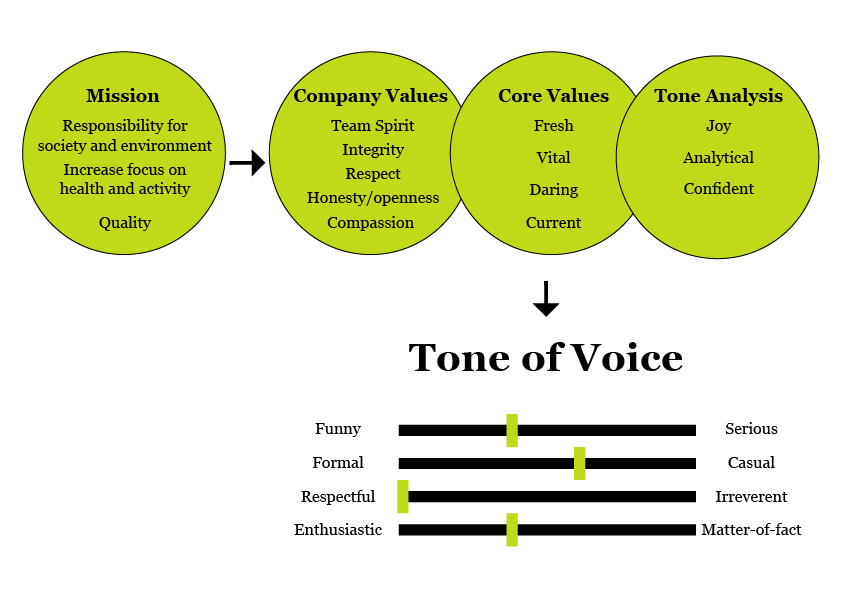
\includegraphics[width=\textwidth]{figures/Tone-of-voice.png}
            \caption{This figure shows how the tone-of-voice was defined by understanding the mission, the values and conducting a tone analysis of the written copy}
            \label{fig:tov}
        \end{figure}
    
        Figure \ref{fig:tov} shows how the tone-of-voice was determined by assessing the mission statement, the company's values inwards and outwards, and through a tone analysis. The tone analysis was conducted using the IBM tone analyser of the written copy found on the brands website. Their tone-of-voice as reflected in their copy is more serious than funny, but not too serious as the tone is also a nice in-between of formal and casual. Their tone is very respectful, which follows their core values of tolerance and respectfulness. Lastly they are leaning towards more enthusiastic than matter-of-fact as they carry a very positive and joyful view of the future and their path to fulfill their goals.

        In addition to the tone-of-voice analysis as proposed by Norman and Nielsen, IBM’s tone analyser tool was also applied to look more into the “mood” they come across as through their web content. The tone analyser searches through content looking for certain words, sentences and phrases that would indicate the mood of the person writing the copy. Their analysis identifies the tones or emotions/mood: anger, fear, joy, sadness, analytical, confident, and tentative. The sentences are then scored and sorted based on how strong they are. If more than one tone is identified in a sentence, then the stronger it is ranked. Four of the tones were identified consistently through the content:
    
        \begin{enumerate}
            \item Analytical
            \item Joy
            \item Confidence
            \item Tentative
        \end{enumerate}

        IBM’s Tone Analyser tool revealed that the tone represented in its online copy consists of: Joy, Analytical, and Confident. In some areas it is also identified as tentative because they are careful in making broad assumptions about its brand: ”We are probably the biggest supplier in Norway”. Rather than tentative a more befitting trait would be humble or realistic. Joy covers any copy where they talks about its achievements, goals and mission - they have a positive outlook and take pride in their achievements towards a healthier population. Analytical is identified where they use numbers and facts to describe their mission and why consumers can trust in their freshness and quality - this is their seriousnesses in regards to who they are and what they aim to achieve - goal driven and intellectual attitude. Confidence is shown through assertiveness and certainty - they are certain they are on the right path to achieve their goals, and they know that they can help people change. 


    \subsection{Implementation phase}
        \subsection{Conversational Design}
        \subsection{Avatars}
    
    \vspace{5mm} %5mm vertical space
    
    \section{Experiment Setup}
    
    A scenario based test was constructed in order to test the personality of the chatbot and whether the personality affects the user experience. The users will be given a series of tasks testing the most important requirements of the system as revealed through the design process. The test will be used to assess whether the personality is perceived as consistent for all users by implementing the Agree! evaluation method in which compares the given characteristics and personality traits with the agreement of users. The the user experience will be measured by using the Attrakdiff questionnaire to assess the usability and design. 
    
    \vspace{5mm} %5mm vertical space

    \subsection{Hypotheses}
 
    \begin{itemize}
         \item \textit {H11: Chatbot A will have a positive effect on the user experience}
        \item \textit {H10: Personality has no effect on the user experience of chatbots}
            \vspace{5mm} %5mm vertical space

        \item \textit {H21: Users will perceive chatbot A as more consistent than chatbot B}
        \item  \textit {H20: Users will not perceive chatbot A as more or less consistent than chatbot B} 
            \vspace{5mm} %5mm vertical space

        \item \textit {H31: Users will perceive chatbot A more positively than chatbot B}
        \item \textit {H30: Users will not perceive chatbot A more or less positively than chatbot B}
    \end{itemize}
    
    \vspace{5mm} %5mm vertical space
    
    \subsection{Data Collection}
    
    \vspace{5mm} %5mm vertical space

     \subsubsection{Agree!}
     
     In order to evaluate whether the personality is perceived consistently, the participants will be asked to describe the personality in relation to predefined characteristics that are compatible with the chosen personality. The participants will be given a set of characteristics and rate them on whether they perceived or did not perceive that characteristic when interacting with the chatbot. The evaluation will be conducted using the Agree! Tool. This is a software developed by Callejas (2014) that implements the framework for the assessment of synthetic personalities. %site website. 
     
     According to Callejas (2014) Agree! will help evaluate personality in three main dimensions:
    
        \begin{itemize}
            \item Whether the rendered personality is perceived by the users as the designers intended. For example, if the designers plan an extrovert personality, whether users perceive it as extrovert or as something else.
            \item Whether the personality is recognizable, that is, if users perceive it consistently (i.e. if users agree in their perceptions, or different users perceive very different personalities).
            \item Whether the agent's personality matches the users' personality, and how the previous dimensions are affected by the personality of users.
        \end{itemize}
            
    \vspace{5mm} %5mm vertical space
   
     \subsubsection{Attrakdiff}
    
    In order to collect the appropriate data from the test, the Attrakdiff questionnaire was used to assess and compare the two chatbot prototypes. The Attrakdiff assesses personal user rating of a products usability and design. It is an evaluation method that records both the perceived pragmatic quality, the hedonic quality and the attractiveness of an interactive product (cite).
    
        \begin{itemize}
            \item Pragmatic Quality: Usefulness and usability of the system
            \item Hedonic Quality: Motivation, stimulation and challenge for the user
        \end{itemize}
    

   
\chapter{Results}
\label{chap:results}

This section will provide the results from the data analysis of both parts of the experiment; 1) the agreement regarding the personality traits and characteristics, 2) the AttrakDiff evaluation to assess the user experience. The data was analysed using SPSS.

\section{Part 1 Results: Personality characteristics data analysis}

The characteristics were rated using a scale from 1-5 in which 5 meant a high perceived presence of the characteristic in the interaction with the chatbots, and 1 meant no perceived presence of the characteristics. The data-set was analysed through running a paired-samples t-test, and a two-way repeated measures ANOVA to investigate whether an interaction effect occurred within subjects, as all participants were subjected to all conditions. The analysis performed on this data set will be used to test $H_1 1$: \textit{Users will perceive the personality of Chatbot A as different to the personality of Chatbot B}, $H_1 2$: \textit{Users will perceive the personality of Chatbot A as intended}, and $H_1 3$: \textit{Users will perceive the personality of Chatbot B as intended}. The descriptive statistics of the characteristics data analysis can be found in table \ref{table:5}.

\begin{table}[h]
\centering
\begin{tabular}{lccccc}
\hline
\multicolumn{6}{c}{\textbf{Descriptive Statistics}} \\
\hline
& N & Minimum & Maximum & Mean & Std. Deviation \\
$Extroversion_A$ & 16 & 2 & 5 & 4,3125 & 0,8116 \\
$Extroversion_B$ & 16 & 1,67 & 3,33 & 2,2708 & 0,47483 \\
$Agreeable_A$ & 16 & 4 & 5 & 4,625 & 0,30277 \\
$Agreeable_B$ & 16 & 2,25 & 4,5 & 3,4219 & 0,57532 \\
$Conscientious_A$ & 16 & 3,33 & 5 & 4,2917 & 0,5146 \\
$Conscientious_B$ & 16 & 2,67 & 4,67 & 3,9167 & 0,60246 \\
$Openness_A$ & 16 & 3 & 5 & 4,0781 & 0,59665 \\
$Openness_B$ & 16 & 1,5 & 5 & 3,4531 & 0,92294 \\
\end{tabular}
 \caption{Descriptive statistics chatbot characteristics results}
 \label{table:5}
    \end{table}

The two-way repeated measures ANOVA examined whether the starting condition had an interaction effect. The independent variable personality has two levels, and the dependent variable characteristics has four factors where each factor describes a factor from the five factor model (extroversion, agreeable, conscientiousness, openness). The two-way repeated ANOVA included a starting condition (startbot) to investigate whether the order of chatbots participants were subjected to had any effect on the results.

There was a significant main effect of the two levels of personality with respect to the characteristics F(1,14)=73,181, p<,001. There was also a significant main effect between the characteristics F(3,42)=12,960, p<,001. There was an INsignificant interaction effect of the starting condition (personality*characteristics*startbot) p=,380. See figure \ref{fig:characstartAB}.

\begin{figure}[h]
    \centering
    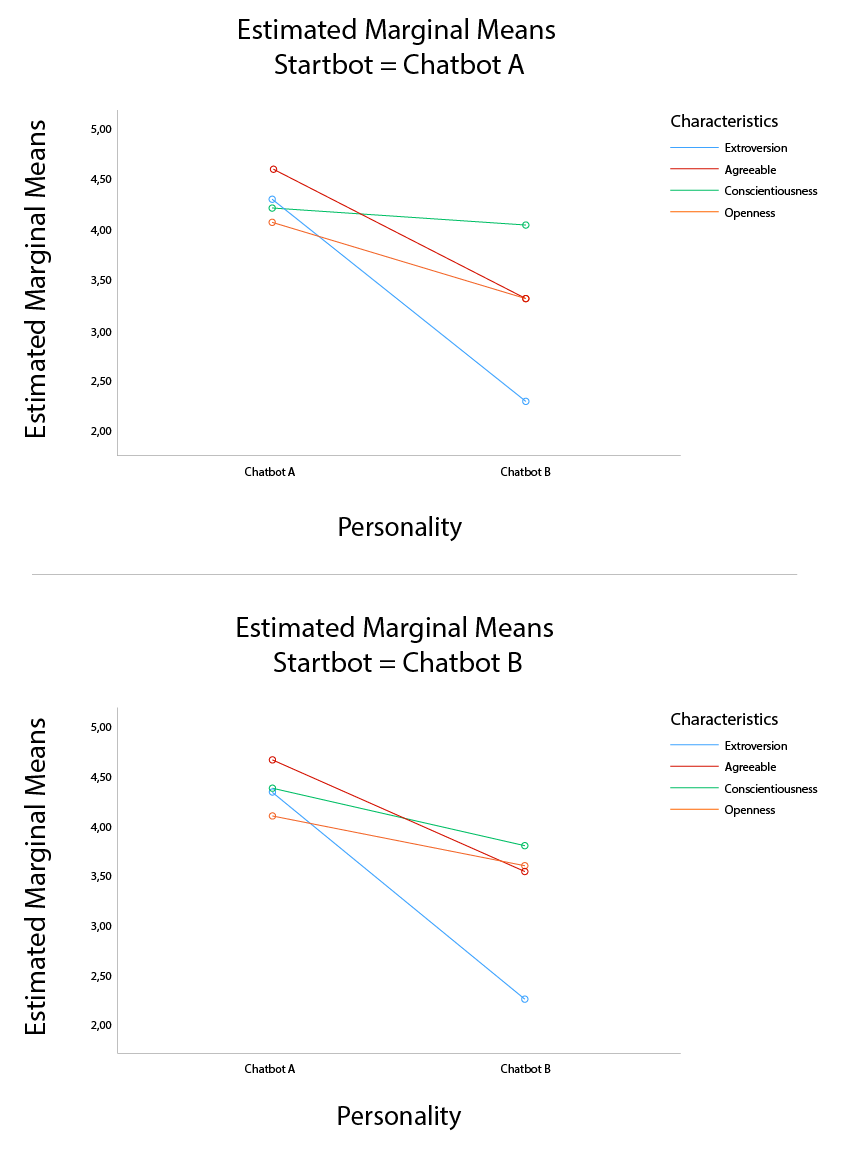
\includegraphics[scale=0.4]{figures/MMeanStartbotABCharacteristics.png}
    \caption{Estimated marginal means of characteristics starting condition Chatbot A and Chatbot B}
    \label{fig:characstartAB}
\end{figure}

\begin{figure}
    \centering
    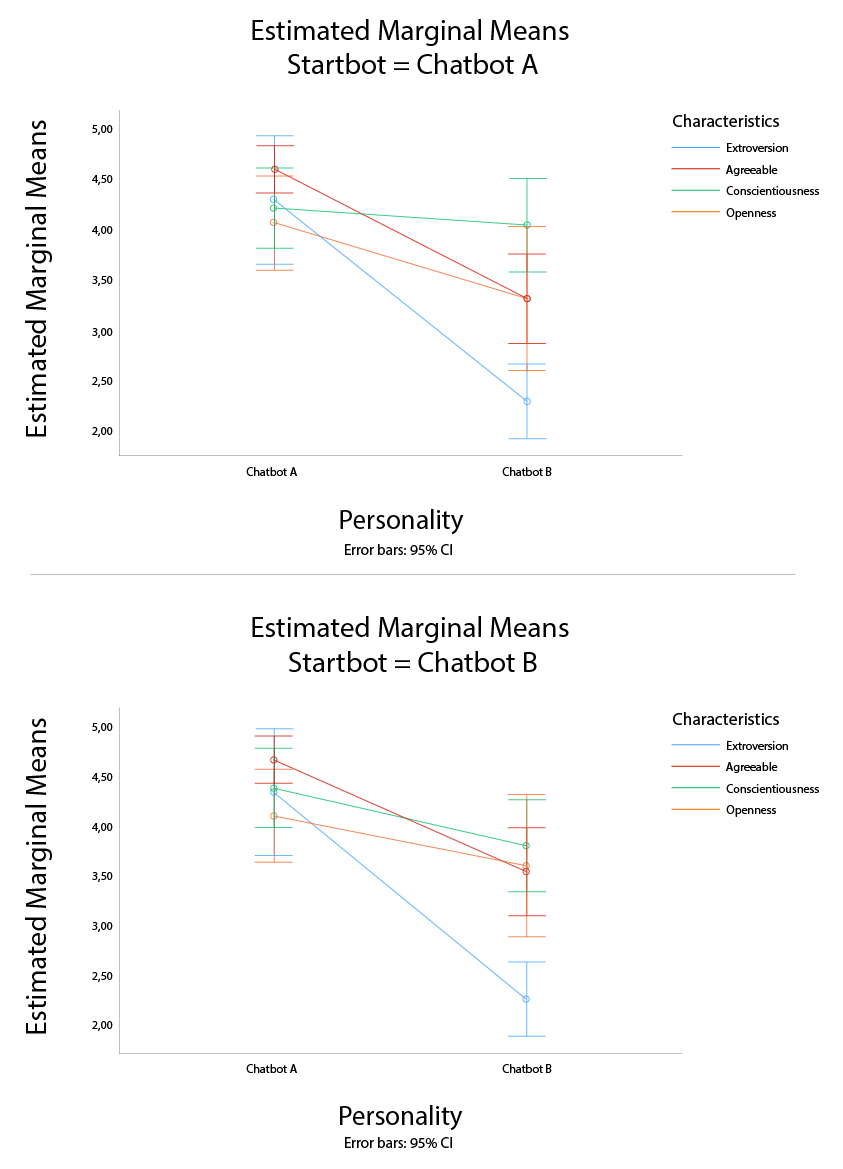
\includegraphics[scale=0.4]{figures/Errorbars_characertistics.png}
    \caption{Estimated marginal means of characteristics starting condition Chatbot A and Chatbot B with Error bars: 95\% CI}
    \label{fig:errorCh}
\end{figure}

The data was also tested for whether there was an interaction effect of gender. This two-way repeated measures ANOVA revealed no significant interaction effect of gender (Personality*Characteristics*Gender) p=,331.

The paired-samples t-test found that there is a significant difference between the two levels of personality and the perceived characteristics. Agreeableness Chatbot B (M=3,4219, SD=,57532) and Agreeableness Chatbot A (M=4,6250, SD=,30277); t(15)=-8,760, p < ,001. Extroversion Chatbot B (M=2,2708, SD=,47483) and Extroversion Chatbot A (M=4,3125, SD=,81166) t(15)=-8,976, p < ,001. Openness Chatbot B (M=3,4531, SD=,92294) and Openness Chatbot A (M=4,0781 SD=,59665) t(15)=-3,727, p = ,002. Conscientiousness Chatbot B (M=3,9167, SD=,60246) and Conscientiousness Chatbot A (M=4,2917, SD=,51460) t(15)=-2,522, p = ,023. These results suggests that participants perceived the two personalities as significantly different from one another. The Mean score difference between Chatbot B and A, suggests that participants perceived all characteristics in Chatbot A to a higher degree than in Chatbot B, where the extroversion factor had the largest difference in mean score.

\section{Part 2 Results: AttrakDiff data analysis }
        
The results from the AttrakDiff evaluation was also analysed by running a paired samples t-test, and a two-way ANOVA to understand whether any interaction effects occurred. The statistics will be used to test $H_1 4$: \textit{Personality affects the user experience of chatbots}, and $H_1 5$: \textit{Chatbot A will have an improved effect over Chatbot B}. The descriptive statistics of the AttrakDiff data analysis can be found in table \ref{table:6}. Descriptive statistic for all word-pairs found in each factor can be found in Appendix \todo{appendix}.

\begin{table}[h]
\centering
\begin{tabular}{lccccc}
\hline
\multicolumn{6}{c}{\textbf{Descriptive Statistics}} \\
\hline
& N & Minimum & Maximum & Mean & Std. Deviation \\
$PQ_A$ & 16 & 4,86 & 6,71 & 5,9286 & 0,56424 \\
$PQ_B$ & 16 & 4 & 6,43 & 5,4732 & 0,5964 \\
$HQ-I_A$ & 16 & 4 & 6,29 & 5,4821 & 0,53165 \\
$HQ-I_B$ & 16 & 3,57 & 5,43 & 4,7679 & 0,56874 \\
$HQ-S_A$ & 16 & 5,14 & 6,14 & 5,625 & 0,29909 \\
$HQ-S_B$ & 16 & 2,57 & 6,57 & 4,7768 & 1,19405 \\
$ATT_A$ & 16 & 5,14 & 7 & 6,3482 & 0,44864 \\
$ATT_B$ & 16 & 3,9 & 6,3 & 5,339 & 0,7805 \\
\end{tabular}
\caption{Descriptive statistics AttrakDiff results}
 \label{table:6}
    \end{table}

A two-way repeated measures ANOVA was conducted to investigate the effect the starting condition (startbot) had on the independent variable personality and the dependent variable user experience. Personality has two levels (personality, no personality) and user experience has four factors (pragmatic, hedonic stimulation, hedonic identity, attractiveness). The between-subjects factor (startbot), tested for any interaction effect dependent on which chatbot participants started with (chatbot A or Chatbot B).

There was a significant main effect of the two levels of personality with respect to the user experience F(1,14)=15,300, p=,002), and the starting condition (startbot) had no significant interaction effect on personality p=,847. There was a significant main effect of the user experience F(3,42)=12,264, p<,001, and the starting condition (startbot) had no significant interaction effect on user experience p=,865. There was no significant interaction effect between personality, user experience and starting condition (personality*UXscore*startbot) p=,909. See figure \ref{fig:startA} and \ref{fig:startB}.

\begin{figure}[h]
    \centering
    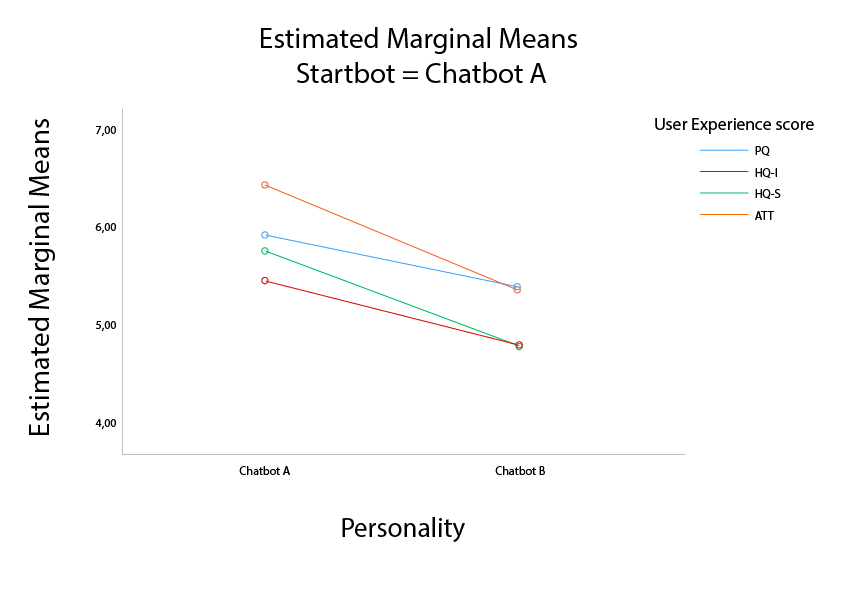
\includegraphics[scale=0.4]{figures/MMeanStartbotA.png}
    \caption{Estimated marginal means starting condition chatbot A user experience score}
    \label{fig:startA}
\end{figure}

\begin{figure}
    \centering
    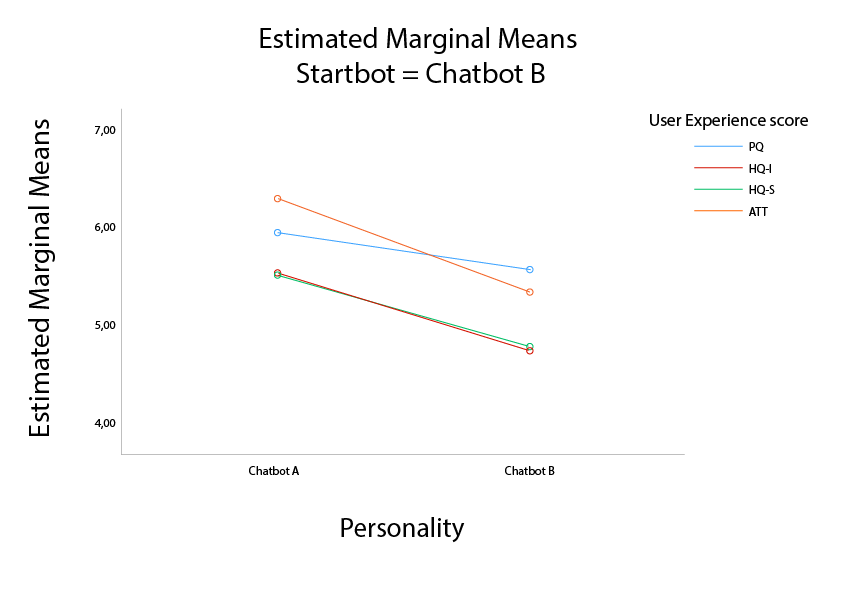
\includegraphics[scale=0.4]{figures/MMeanStartbotB.png}
    \caption{Estimated marginal means starting condition chatbot B user experience score}
    \label{fig:startB}
\end{figure}

\begin{figure}
    \centering
    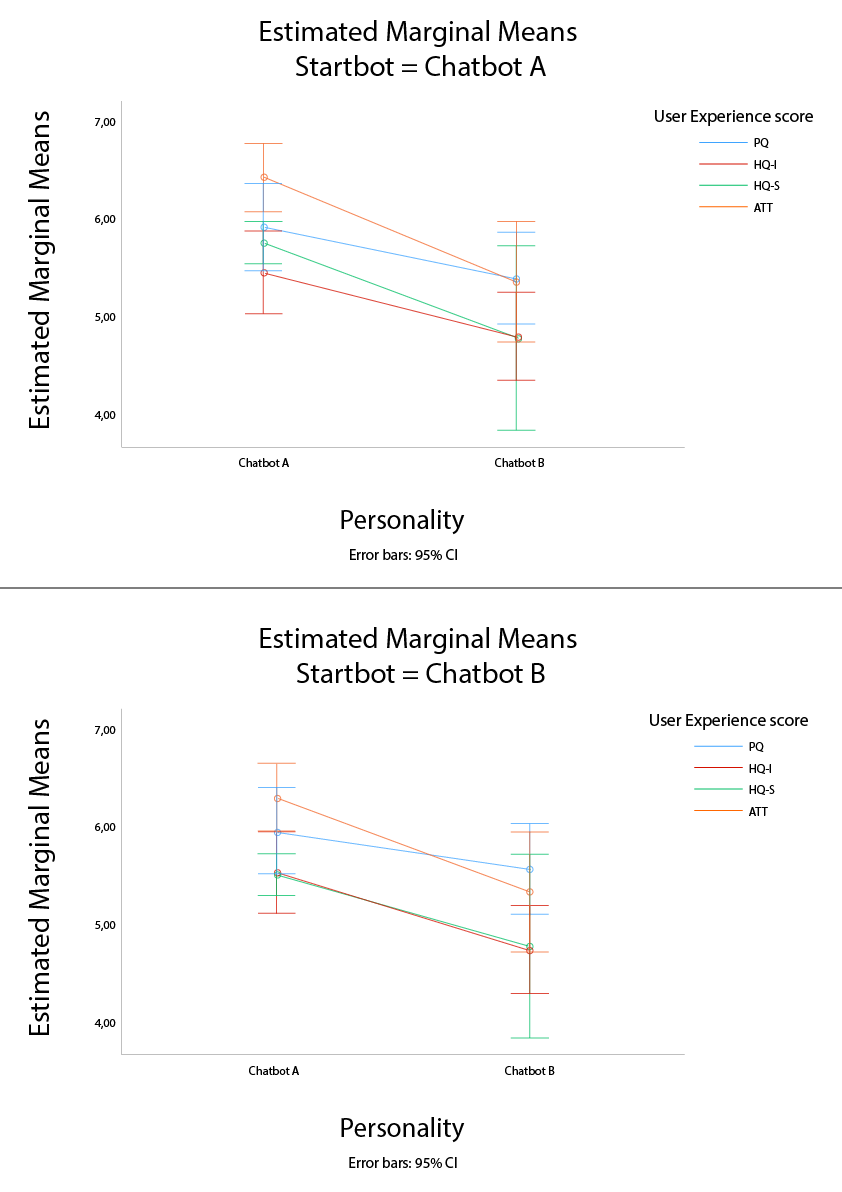
\includegraphics[scale=0.4]{figures/ErrorBarsStartbotAB.png}
    \caption{Estimated marginal means of user experience score starting condition Chatbot A and Chatbot B with Error bars: 95\% CI}
    \label{fig:errorUX}
\end{figure}

Another two-way repeated measures ANOVA was conducted to investigate whether gender had any significant interaction effect on the variables. The analysis found that there was no significant interaction effect between personality, user experience and gender (personality*UXscore*gender) p=,436.

The paired samples t-test found that there is a significant difference in the scores between Chatbot B and Chatbot A, where all four factors of the user experience showed a significant improved effect between Chatbot B and A. Pragmatic Quality Chatbot B (M=5,4732, SD=,59649) and Pragmatic Quality Chatbot A (M=5,9286, SD=56424); t(15)=-2,152, p = ,048. Hedonic-I Quality Chatbot B (M=4,7679, SD=,56874) and Hedonic-I Quality Chatbot A (M=5,4821, SD=,53165) t(15)=-3,239, p = ,006. Hedonic-S Quality Chatbot B (M=4,7768, SD=1,19405) and Hedonic-S Quality Chatbot A (M=5,6250 SD=,29909) t(15)=-2,934, p = ,010. Attractiveness Chatbot B (M=5,339, SD=,7805) and Attractiveness Chatbot A (M=6,3482, SD=,44864) t(15)=-4,069, p = ,001. These results suggests that personality has an improved effect on the user experience of chatbots, as all four factors of user experience was scored higher for Chatbot A than Chatbot B.

\begin{figure}[h]
    \centering
    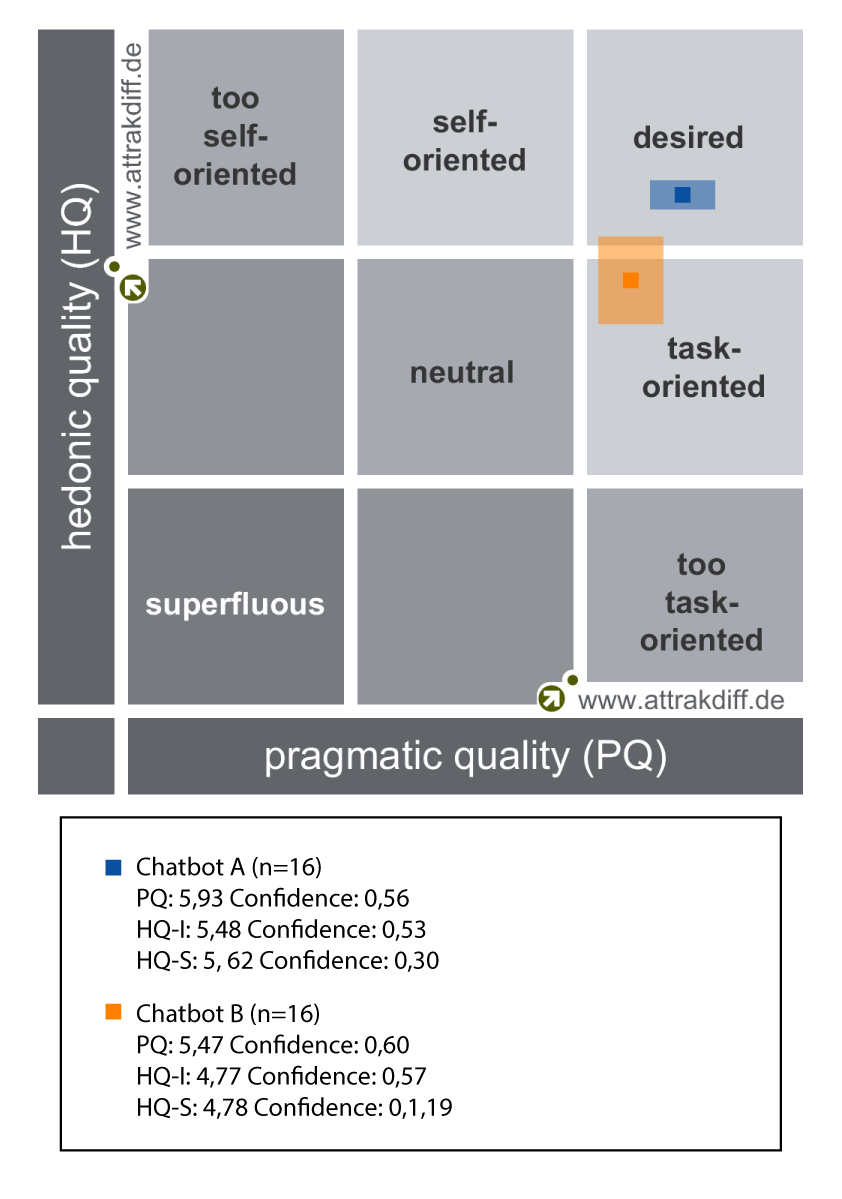
\includegraphics[scale=0.4]{figures/Portfolio-of-results-attrakdiff.png}
    \caption{Results Attrakdiff}
    \label{fig:portres}
\end{figure}
        
As shown in Figure \ref{fig:portres}, Chatbot A performed better in both hedonic and pragmatic quality than Chatbot B. The rectangles shows the confidence observed for Chatbot A and B, where Chatbot A has a smaller confidence rectangle implying that the participants were largely at one. Chatbot B however has a much larger confidence rectangle, which suggests that participant responses differed more greatly. Figure \ref{fig:diagval} shows the mean score of each user experience factor and how the two personalities scored compared to each other. The diagram shows that the difference is greater when it comes to hedonic quality-simulation and attractiveness, while the differences are less when it comes to pragmatic quality in particular. As the two personalities only shared traits found in the conscientiousness personality factor (reliable, consistent, perceptive) this result is to be expected as those traits are often found to be pragmatic qualities. Figure \ref{fig:wordpairs} shows the average score for each of the word-pairs for both chatbot versions. This line graph shows clearly where the differences are largest, such as human-technical, and that for the majority of word-pairs Chatbot A scores higher. The exceptions includes mainly word-pairs in the pragmatic quality: cumbersome-straightforward, unpredictable-predictable, unprofessional-professional. This suggests that a technical, impersonal or machine-like personality are seen as more professional and straightforward than a more human-like personality.

\begin{figure}[h]
    \centering
    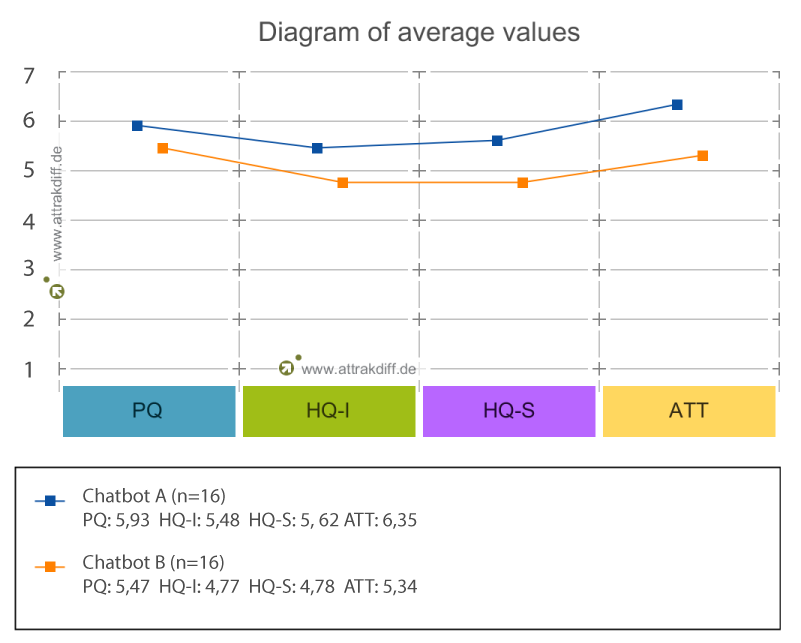
\includegraphics[scale=0.5]{figures/Diagram-of-average-values.png}
    \caption{Diagram of average values}
    \label{fig:diagval}
\end{figure}

\begin{figure}[h]
    \centering
    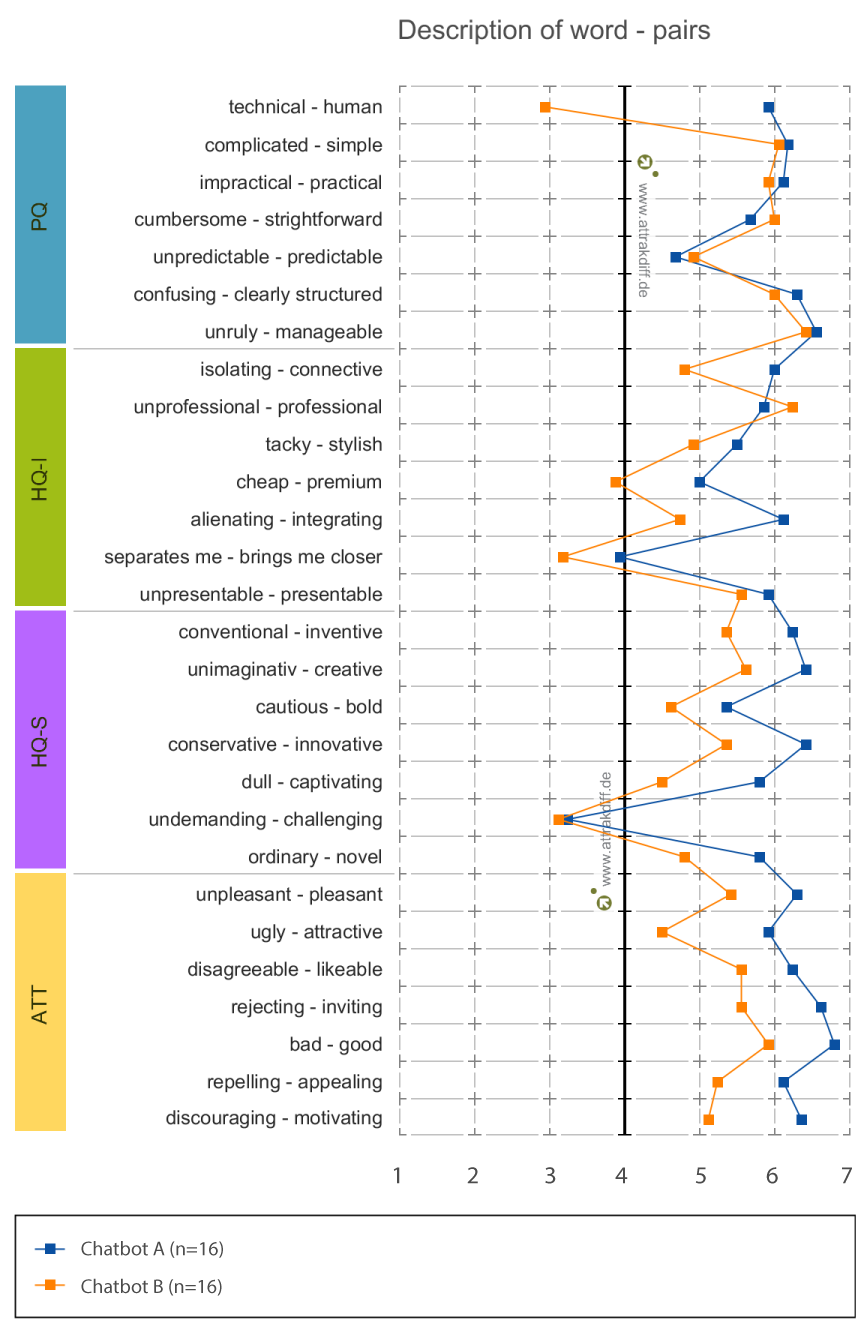
\includegraphics[scale=0.4]{figures/Description-of-word-pairs.png}
    \caption{Description of word-pairs}
    \label{fig:wordpairs}
\end{figure}
\chapter{Discussion}
\label{chap:discussion}

The results you have collected and the process you when through to develop the project have been presented earlier.  This Chapter is used to talk about your interpretations of results or the process.  It might be a discussion of the language you used.  A tool that you started to use but then stopped using for some reason.  It could give insight into the evolution of your process.

Future research:

Use the agree framework for actively when testing the personality. The framework is built on participants interacting with a chatbot in a series of interactions where there is a change in attitude (e.g. unfriendly, neutral, friendly). Instead of testing the change in attitude in this project, participants will instead be asked to rate on a Likert scale to what extent they perceived the specific traits.

\todo{ give more examples of discussions}
\chapter{Conclusion}
\label{chap:conclusion}

This is where you provide an overview of the thesis now that it is finished.  What are the critical things that can be learnt from the thesis for the reader.

This is additional text.

\section{Future Work}
\label{sec:future}
Where would the project go from here.

\todo{again more examples and discussion about what it means to plan}

\todo{there are many more things to say}
\chapter{Packages}
\label{chap:packages}

The \texttt{ntnuthesis} is built upon the standard \LaTeX\
\texttt{report} class. All commands from the \texttt{report} class can
be used, with the two exceptions of \verb+\subsubsection+ and
\verb+\paragraph+. This is because there should only be three
levels of headings according to the guidelines. 
It has been placed in a folder called \texttt{ntnuthesis} so that it does not
clutter your work.  You should not change anything in \texttt{ntnuthesis}. If you need to change 
anything you should make a pull request on the github repository for this thesis at
\url{https://github.com/COPCSE-NTNU/master-theses-NTNU}

\section{Packages Used by ntnuthesis}
\label{sec:packages}

In addition to the \texttt{report} document class,
\texttt{ntnuthesis} makes direct use of the following packages
that must hence be present:
\begin{description}
	\item[geometry:] used for setting the sizes of the margins and
  	headers.
	\item[fontenc:] used with option \texttt{T1} for forcing the Cork font
  	encoding (necessary for the Charter font).
	\item[charter:] load Charter as the default font.
	\item[euler:] load the Euler math fonts.
	\item[bable:] for language handling.
	\item[listing:] for code listing.
\end{description}

\section{Other Relevant Packages}
\label{sec:otherpackages}

The author of a thesis might want to use a bunch of different packages
to those described in Section~\ref{sec:packages} in order to have all features needed for their document. 
In particular, it is advised to use the following:
\begin{description}
	\item[inputenc:] to allow \LaTeX\ to use more than 7-bit ASCII for its
	  input. Most often, the option \texttt{latin1} will do.
	\item[babel:] to load language specific strings. Reasonable options
	  include \texttt{british}, 
		\texttt{american}, \texttt{norsk} and
	  \texttt{nynorsk}.
	\item[graphicx:] to include graphics.
	\item[hyperref:] this is a very nice package that makes cross links in
	  pdf documents. Use with option \texttt{dvips} or \texttt{pdftex}
	  in accordance with the driver that you use. Unfortunately, hyperref
	  is not completely bugfree\dots
\end{description}

We have web pages as well~\cite{NTNU:Website}, and now games like Halo~\cite{Halo}. % could be called Methodology or methods or any filename 
\chapter{Structural Elements}
\label{chap:structural}

If you are submitting using the DAIM system you should make sure the pdf you submit does not have the front page information, as that will be added by the submission form in DAIM.  You can remove the DAIM option to print the front page material if you want a full PDF with the front page material. To make sure the running header has the title of the thesis you still need to set it in the \verb+DaimData.tex+ file. The title of the thesis should be set using the \verb+\thesistitle+
command, and the date of the thesis should be set using the
\verb+\thesisdate+ command in the \verb+DaimData.tex+ file. 

\section{Page Layout}

The geometry of the page has been set using the \verb+\geometry+
command.

\section{Fonts}

Due to limited \LaTeX\ support for the Georgia font, Charter has been
chosen instead. For mathematical formula, the Euler fonts are used,
since they blend more nicely with the Charter than the standard
\LaTeX\ fonts: 
\begin{equation} \label{eq:1}
    f(x) = \int_0^x g(\tau)\,d\tau
\end{equation}



For inline math you can use $\backslash{}($ and $\backslash{})$ for example \( f(x)= \frac{x^2}{1+x^2} \).  
This also allows you to use $\slash$ and $\backslash$. You need to include the \{\} when you want the special
character to have other letters immediately after it.

\section{Sectioning Commands}

The standard \LaTeX\ sectioning commands are used for both numbered
and unnumbered sections. The top level is given by the \verb+\chapter+
command. This starts a new right page. The two lower levels are
obtained using the \verb+\section+ and \verb+\subsection+ commands.
The standard \LaTeX\ \verb+\subsubsection+ and \verb+\paragraph+
commands have been disabled since their use is not encouraged by the
thesis guidelines. When you use these they will not be given numbers.  
They still appear in the document with highlighting but not in the 
table of contents.

\subsection{The subsection}

This is an example of a subsection.

\subsubsection{The subsubsection}

This is an example of a subsubsection.

\paragraph{The paragraph}

This is an example of a paragraph with a heading.

\section{Floats (Figures and Tables)}
\label{sec:floats}

Figures are placed in the \texttt{figure} environment. An example is
shown in Figure~\ref{fig:example}. %notice the ~ in between figure and the \ref. it stops latex from splitting the number and word over a line.
Tables are placed in the \texttt{table} environment. An example is given in
Table~\ref{tab:example} and reading the information directly from file in Table~\ref{tab:examplecsv}. Figures and tables float freely around in the
document in accordance with standard \LaTeX\ behavior.

\begin{figure}[tbp]  %t top, b bottom, p page | you can also use h to try to get the figure to appear at the current location
  \centering
  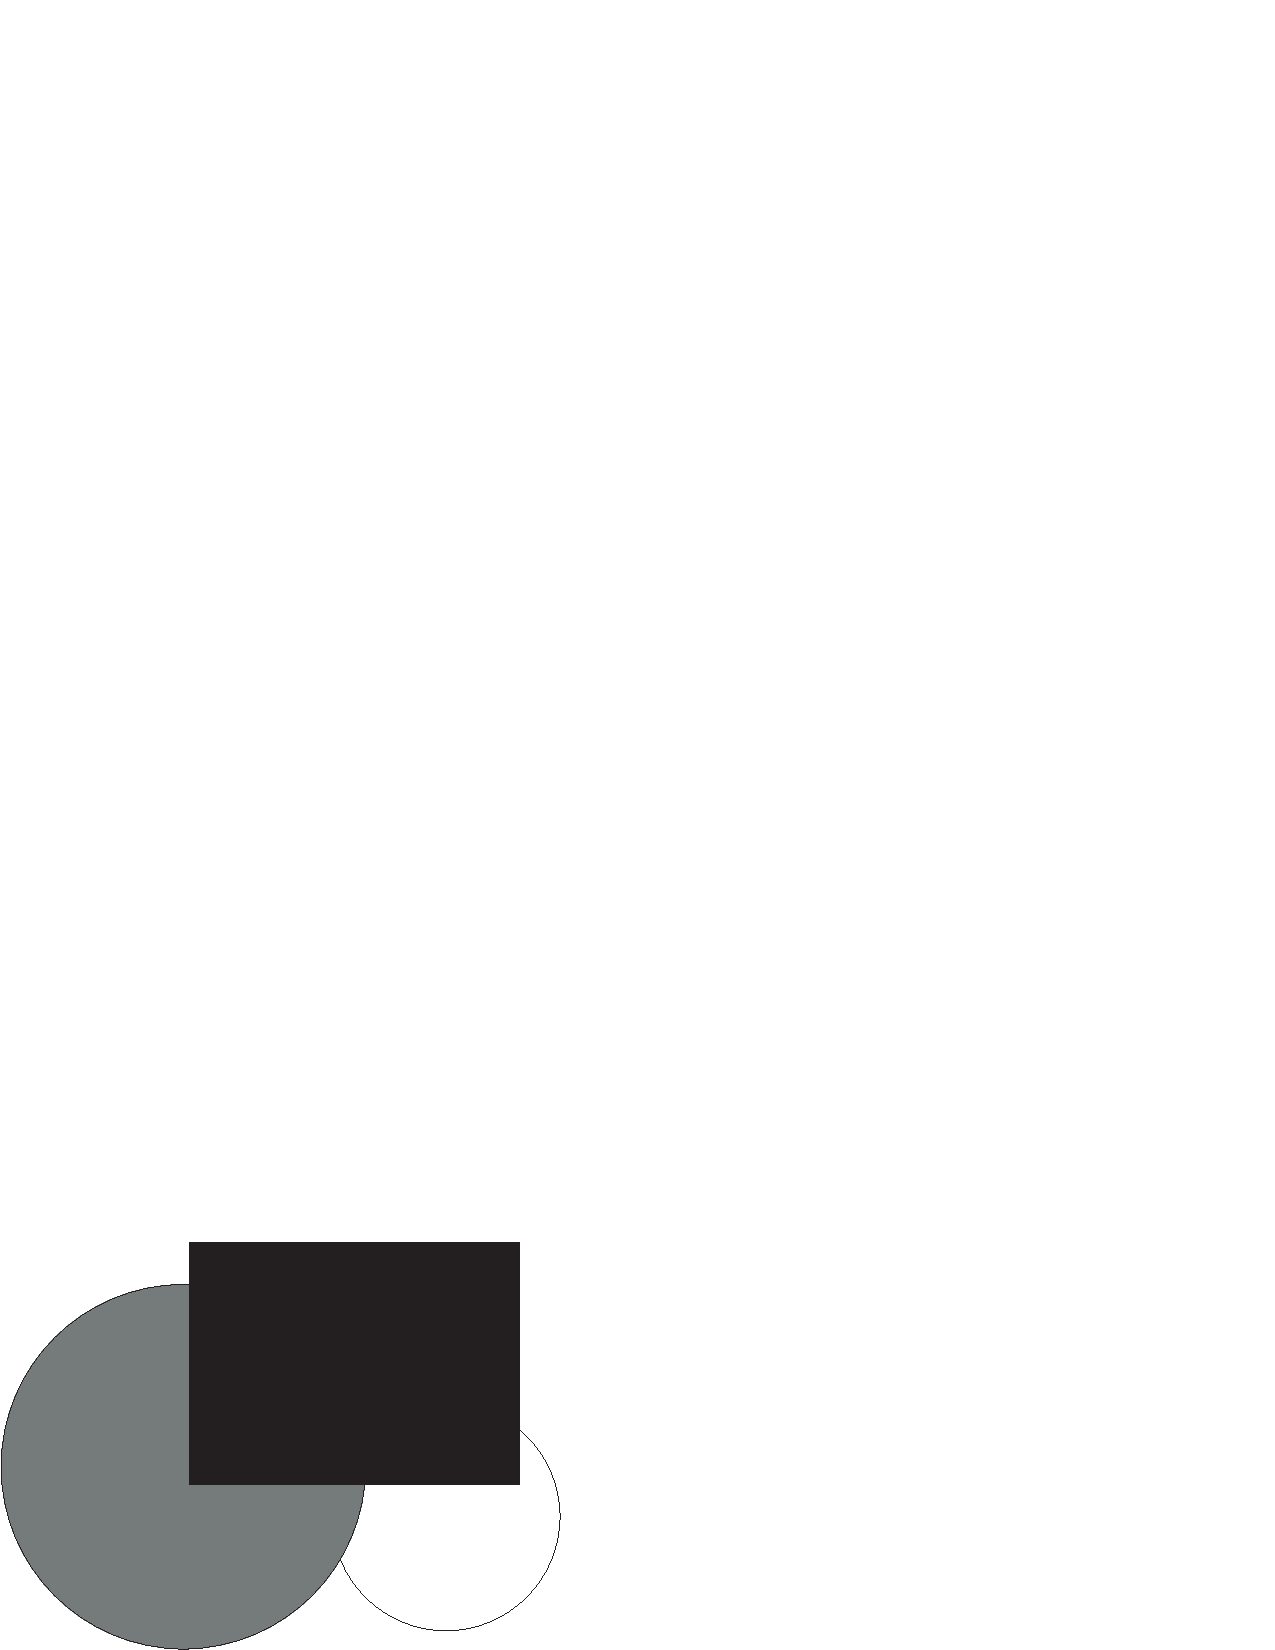
\includegraphics[width=.5\textwidth]{figures/example_fig}
  \caption[An example figure.]{An example figure. If the caption is
    shorter than one line, it is centered. If it goes over more than
    one line, it is left and right justified. Furthermore, it is
    suggested that an alternative short caption is given in order to
    produce a good list of figures.}
  \label{fig:example}
\end{figure}

\begin{table}[tbp]
  \centering
  \begin{tabular}{c|c}
    Age  & IQ  \\ 
    \hline
    10   & 100 \\
    20   & 100 \\
    30   & 150 \\
    40   & 100 \\
    50   & 100
  \end{tabular}
  \caption{An example table.}
  \label{tab:example}
\end{table}

\begin{table}[tbp]
  \centering
  \csvautobooktabular{figures/ageiq.csv}
  \caption{An example table using simplecsv.}
  \label{tab:examplecsv}
\end{table}

The captions are placed \emph{below} both for the figures and the
tables. The caption is set in 9pt. If the caption is shorter than one
line, it is centered.

\subsection{Gnuplot}
There are many ways to include graphs in your document.  Figure~\ref{fig:exgnuplotex} for including a file generated by gnuplot and saved as \texttt{gnuplotgraph1.tex}. 
%Figure~\ref{fig:exgnuplotintegrate} shows how to include the script to generate a graph direction in \LaTeX.

\begin{figure}[htp]  %t top, b bottom, p page | you can also use h to try to get the figure to appear at the current location
  \centering
  % GNUPLOT: LaTeX picture
\setlength{\unitlength}{0.240900pt}
\ifx\plotpoint\undefined\newsavebox{\plotpoint}\fi
\begin{picture}(1500,900)(0,0)
\sbox{\plotpoint}{\rule[-0.200pt]{0.400pt}{0.400pt}}%
\put(130.0,82.0){\rule[-0.200pt]{4.818pt}{0.400pt}}
\put(110,82){\makebox(0,0)[r]{-1}}
\put(1419.0,82.0){\rule[-0.200pt]{4.818pt}{0.400pt}}
\put(130.0,151.0){\rule[-0.200pt]{4.818pt}{0.400pt}}
\put(110,151){\makebox(0,0)[r]{-0.8}}
\put(1419.0,151.0){\rule[-0.200pt]{4.818pt}{0.400pt}}
\put(130.0,221.0){\rule[-0.200pt]{4.818pt}{0.400pt}}
\put(110,221){\makebox(0,0)[r]{-0.6}}
\put(1419.0,221.0){\rule[-0.200pt]{4.818pt}{0.400pt}}
\put(130.0,290.0){\rule[-0.200pt]{4.818pt}{0.400pt}}
\put(110,290){\makebox(0,0)[r]{-0.4}}
\put(1419.0,290.0){\rule[-0.200pt]{4.818pt}{0.400pt}}
\put(130.0,360.0){\rule[-0.200pt]{4.818pt}{0.400pt}}
\put(110,360){\makebox(0,0)[r]{-0.2}}
\put(1419.0,360.0){\rule[-0.200pt]{4.818pt}{0.400pt}}
\put(130.0,429.0){\rule[-0.200pt]{4.818pt}{0.400pt}}
\put(110,429){\makebox(0,0)[r]{ 0}}
\put(1419.0,429.0){\rule[-0.200pt]{4.818pt}{0.400pt}}
\put(130.0,498.0){\rule[-0.200pt]{4.818pt}{0.400pt}}
\put(110,498){\makebox(0,0)[r]{ 0.2}}
\put(1419.0,498.0){\rule[-0.200pt]{4.818pt}{0.400pt}}
\put(130.0,568.0){\rule[-0.200pt]{4.818pt}{0.400pt}}
\put(110,568){\makebox(0,0)[r]{ 0.4}}
\put(1419.0,568.0){\rule[-0.200pt]{4.818pt}{0.400pt}}
\put(130.0,637.0){\rule[-0.200pt]{4.818pt}{0.400pt}}
\put(110,637){\makebox(0,0)[r]{ 0.6}}
\put(1419.0,637.0){\rule[-0.200pt]{4.818pt}{0.400pt}}
\put(130.0,707.0){\rule[-0.200pt]{4.818pt}{0.400pt}}
\put(110,707){\makebox(0,0)[r]{ 0.8}}
\put(1419.0,707.0){\rule[-0.200pt]{4.818pt}{0.400pt}}
\put(130.0,776.0){\rule[-0.200pt]{4.818pt}{0.400pt}}
\put(110,776){\makebox(0,0)[r]{ 1}}
\put(1419.0,776.0){\rule[-0.200pt]{4.818pt}{0.400pt}}
\put(130.0,82.0){\rule[-0.200pt]{0.400pt}{4.818pt}}
\put(130,41){\makebox(0,0){-10}}
\put(130.0,756.0){\rule[-0.200pt]{0.400pt}{4.818pt}}
\put(457.0,82.0){\rule[-0.200pt]{0.400pt}{4.818pt}}
\put(457,41){\makebox(0,0){-5}}
\put(457.0,756.0){\rule[-0.200pt]{0.400pt}{4.818pt}}
\put(785.0,82.0){\rule[-0.200pt]{0.400pt}{4.818pt}}
\put(785,41){\makebox(0,0){ 0}}
\put(785.0,756.0){\rule[-0.200pt]{0.400pt}{4.818pt}}
\put(1112.0,82.0){\rule[-0.200pt]{0.400pt}{4.818pt}}
\put(1112,41){\makebox(0,0){ 5}}
\put(1112.0,756.0){\rule[-0.200pt]{0.400pt}{4.818pt}}
\put(1439.0,82.0){\rule[-0.200pt]{0.400pt}{4.818pt}}
\put(1439,41){\makebox(0,0){ 10}}
\put(1439.0,756.0){\rule[-0.200pt]{0.400pt}{4.818pt}}
\put(130.0,82.0){\rule[-0.200pt]{0.400pt}{167.185pt}}
\put(130.0,82.0){\rule[-0.200pt]{315.338pt}{0.400pt}}
\put(1439.0,82.0){\rule[-0.200pt]{0.400pt}{167.185pt}}
\put(130.0,776.0){\rule[-0.200pt]{315.338pt}{0.400pt}}
\put(784,838){\makebox(0,0){Test of $y=sin(x)$}}
\put(785,429){\makebox(0,0)[l]{$y=sin(x)$}}
\put(1279,736){\makebox(0,0)[r]{sin(x)}}
\put(1299.0,736.0){\rule[-0.200pt]{24.090pt}{0.400pt}}
\put(130,618){\usebox{\plotpoint}}
\multiput(130.58,609.67)(0.493,-2.439){23}{\rule{0.119pt}{2.008pt}}
\multiput(129.17,613.83)(13.000,-57.833){2}{\rule{0.400pt}{1.004pt}}
\multiput(143.58,546.90)(0.493,-2.677){23}{\rule{0.119pt}{2.192pt}}
\multiput(142.17,551.45)(13.000,-63.450){2}{\rule{0.400pt}{1.096pt}}
\multiput(156.58,479.28)(0.494,-2.553){25}{\rule{0.119pt}{2.100pt}}
\multiput(155.17,483.64)(14.000,-65.641){2}{\rule{0.400pt}{1.050pt}}
\multiput(170.58,408.77)(0.493,-2.717){23}{\rule{0.119pt}{2.223pt}}
\multiput(169.17,413.39)(13.000,-64.386){2}{\rule{0.400pt}{1.112pt}}
\multiput(183.58,340.15)(0.493,-2.598){23}{\rule{0.119pt}{2.131pt}}
\multiput(182.17,344.58)(13.000,-61.577){2}{\rule{0.400pt}{1.065pt}}
\multiput(196.58,274.92)(0.493,-2.360){23}{\rule{0.119pt}{1.946pt}}
\multiput(195.17,278.96)(13.000,-55.961){2}{\rule{0.400pt}{0.973pt}}
\multiput(209.58,216.42)(0.494,-1.892){25}{\rule{0.119pt}{1.586pt}}
\multiput(208.17,219.71)(14.000,-48.709){2}{\rule{0.400pt}{0.793pt}}
\multiput(223.58,165.35)(0.493,-1.607){23}{\rule{0.119pt}{1.362pt}}
\multiput(222.17,168.17)(13.000,-38.174){2}{\rule{0.400pt}{0.681pt}}
\multiput(236.58,125.75)(0.493,-1.171){23}{\rule{0.119pt}{1.023pt}}
\multiput(235.17,127.88)(13.000,-27.877){2}{\rule{0.400pt}{0.512pt}}
\multiput(249.58,97.67)(0.493,-0.576){23}{\rule{0.119pt}{0.562pt}}
\multiput(248.17,98.83)(13.000,-13.834){2}{\rule{0.400pt}{0.281pt}}
\put(262,83.17){\rule{2.700pt}{0.400pt}}
\multiput(262.00,84.17)(7.396,-2.000){2}{\rule{1.350pt}{0.400pt}}
\multiput(275.00,83.58)(0.582,0.492){21}{\rule{0.567pt}{0.119pt}}
\multiput(275.00,82.17)(12.824,12.000){2}{\rule{0.283pt}{0.400pt}}
\multiput(289.58,95.00)(0.493,1.012){23}{\rule{0.119pt}{0.900pt}}
\multiput(288.17,95.00)(13.000,24.132){2}{\rule{0.400pt}{0.450pt}}
\multiput(302.58,121.00)(0.493,1.527){23}{\rule{0.119pt}{1.300pt}}
\multiput(301.17,121.00)(13.000,36.302){2}{\rule{0.400pt}{0.650pt}}
\multiput(315.58,160.00)(0.493,1.924){23}{\rule{0.119pt}{1.608pt}}
\multiput(314.17,160.00)(13.000,45.663){2}{\rule{0.400pt}{0.804pt}}
\multiput(328.58,209.00)(0.494,2.113){25}{\rule{0.119pt}{1.757pt}}
\multiput(327.17,209.00)(14.000,54.353){2}{\rule{0.400pt}{0.879pt}}
\multiput(342.58,267.00)(0.493,2.558){23}{\rule{0.119pt}{2.100pt}}
\multiput(341.17,267.00)(13.000,60.641){2}{\rule{0.400pt}{1.050pt}}
\multiput(355.58,332.00)(0.493,2.717){23}{\rule{0.119pt}{2.223pt}}
\multiput(354.17,332.00)(13.000,64.386){2}{\rule{0.400pt}{1.112pt}}
\multiput(368.58,401.00)(0.493,2.757){23}{\rule{0.119pt}{2.254pt}}
\multiput(367.17,401.00)(13.000,65.322){2}{\rule{0.400pt}{1.127pt}}
\multiput(381.58,471.00)(0.493,2.677){23}{\rule{0.119pt}{2.192pt}}
\multiput(380.17,471.00)(13.000,63.450){2}{\rule{0.400pt}{1.096pt}}
\multiput(394.58,539.00)(0.494,2.333){25}{\rule{0.119pt}{1.929pt}}
\multiput(393.17,539.00)(14.000,59.997){2}{\rule{0.400pt}{0.964pt}}
\multiput(408.58,603.00)(0.493,2.241){23}{\rule{0.119pt}{1.854pt}}
\multiput(407.17,603.00)(13.000,53.152){2}{\rule{0.400pt}{0.927pt}}
\multiput(421.58,660.00)(0.493,1.845){23}{\rule{0.119pt}{1.546pt}}
\multiput(420.17,660.00)(13.000,43.791){2}{\rule{0.400pt}{0.773pt}}
\multiput(434.58,707.00)(0.493,1.408){23}{\rule{0.119pt}{1.208pt}}
\multiput(433.17,707.00)(13.000,33.493){2}{\rule{0.400pt}{0.604pt}}
\multiput(447.58,743.00)(0.494,0.827){25}{\rule{0.119pt}{0.757pt}}
\multiput(446.17,743.00)(14.000,21.429){2}{\rule{0.400pt}{0.379pt}}
\multiput(461.00,766.58)(0.652,0.491){17}{\rule{0.620pt}{0.118pt}}
\multiput(461.00,765.17)(11.713,10.000){2}{\rule{0.310pt}{0.400pt}}
\multiput(474.00,774.93)(1.378,-0.477){7}{\rule{1.140pt}{0.115pt}}
\multiput(474.00,775.17)(10.634,-5.000){2}{\rule{0.570pt}{0.400pt}}
\multiput(487.58,768.29)(0.493,-0.695){23}{\rule{0.119pt}{0.654pt}}
\multiput(486.17,769.64)(13.000,-16.643){2}{\rule{0.400pt}{0.327pt}}
\multiput(500.58,748.50)(0.493,-1.250){23}{\rule{0.119pt}{1.085pt}}
\multiput(499.17,750.75)(13.000,-29.749){2}{\rule{0.400pt}{0.542pt}}
\multiput(513.58,715.37)(0.494,-1.599){25}{\rule{0.119pt}{1.357pt}}
\multiput(512.17,718.18)(14.000,-41.183){2}{\rule{0.400pt}{0.679pt}}
\multiput(527.58,669.82)(0.493,-2.083){23}{\rule{0.119pt}{1.731pt}}
\multiput(526.17,673.41)(13.000,-49.408){2}{\rule{0.400pt}{0.865pt}}
\multiput(540.58,615.67)(0.493,-2.439){23}{\rule{0.119pt}{2.008pt}}
\multiput(539.17,619.83)(13.000,-57.833){2}{\rule{0.400pt}{1.004pt}}
\multiput(553.58,553.03)(0.493,-2.638){23}{\rule{0.119pt}{2.162pt}}
\multiput(552.17,557.51)(13.000,-62.514){2}{\rule{0.400pt}{1.081pt}}
\multiput(566.58,486.28)(0.494,-2.553){25}{\rule{0.119pt}{2.100pt}}
\multiput(565.17,490.64)(14.000,-65.641){2}{\rule{0.400pt}{1.050pt}}
\multiput(580.58,415.77)(0.493,-2.717){23}{\rule{0.119pt}{2.223pt}}
\multiput(579.17,420.39)(13.000,-64.386){2}{\rule{0.400pt}{1.112pt}}
\multiput(593.58,347.03)(0.493,-2.638){23}{\rule{0.119pt}{2.162pt}}
\multiput(592.17,351.51)(13.000,-62.514){2}{\rule{0.400pt}{1.081pt}}
\multiput(606.58,280.79)(0.493,-2.400){23}{\rule{0.119pt}{1.977pt}}
\multiput(605.17,284.90)(13.000,-56.897){2}{\rule{0.400pt}{0.988pt}}
\multiput(619.58,220.94)(0.493,-2.043){23}{\rule{0.119pt}{1.700pt}}
\multiput(618.17,224.47)(13.000,-48.472){2}{\rule{0.400pt}{0.850pt}}
\multiput(632.58,170.48)(0.494,-1.562){25}{\rule{0.119pt}{1.329pt}}
\multiput(631.17,173.24)(14.000,-40.242){2}{\rule{0.400pt}{0.664pt}}
\multiput(646.58,128.75)(0.493,-1.171){23}{\rule{0.119pt}{1.023pt}}
\multiput(645.17,130.88)(13.000,-27.877){2}{\rule{0.400pt}{0.512pt}}
\multiput(659.58,100.41)(0.493,-0.655){23}{\rule{0.119pt}{0.623pt}}
\multiput(658.17,101.71)(13.000,-15.707){2}{\rule{0.400pt}{0.312pt}}
\multiput(672.00,84.95)(2.695,-0.447){3}{\rule{1.833pt}{0.108pt}}
\multiput(672.00,85.17)(9.195,-3.000){2}{\rule{0.917pt}{0.400pt}}
\multiput(685.00,83.58)(0.704,0.491){17}{\rule{0.660pt}{0.118pt}}
\multiput(685.00,82.17)(12.630,10.000){2}{\rule{0.330pt}{0.400pt}}
\multiput(699.58,93.00)(0.493,0.972){23}{\rule{0.119pt}{0.869pt}}
\multiput(698.17,93.00)(13.000,23.196){2}{\rule{0.400pt}{0.435pt}}
\multiput(712.58,118.00)(0.493,1.448){23}{\rule{0.119pt}{1.238pt}}
\multiput(711.17,118.00)(13.000,34.430){2}{\rule{0.400pt}{0.619pt}}
\multiput(725.58,155.00)(0.493,1.924){23}{\rule{0.119pt}{1.608pt}}
\multiput(724.17,155.00)(13.000,45.663){2}{\rule{0.400pt}{0.804pt}}
\multiput(738.58,204.00)(0.493,2.241){23}{\rule{0.119pt}{1.854pt}}
\multiput(737.17,204.00)(13.000,53.152){2}{\rule{0.400pt}{0.927pt}}
\multiput(751.58,261.00)(0.494,2.333){25}{\rule{0.119pt}{1.929pt}}
\multiput(750.17,261.00)(14.000,59.997){2}{\rule{0.400pt}{0.964pt}}
\multiput(765.58,325.00)(0.493,2.717){23}{\rule{0.119pt}{2.223pt}}
\multiput(764.17,325.00)(13.000,64.386){2}{\rule{0.400pt}{1.112pt}}
\multiput(778.58,394.00)(0.493,2.757){23}{\rule{0.119pt}{2.254pt}}
\multiput(777.17,394.00)(13.000,65.322){2}{\rule{0.400pt}{1.127pt}}
\multiput(791.58,464.00)(0.493,2.717){23}{\rule{0.119pt}{2.223pt}}
\multiput(790.17,464.00)(13.000,64.386){2}{\rule{0.400pt}{1.112pt}}
\multiput(804.58,533.00)(0.494,2.333){25}{\rule{0.119pt}{1.929pt}}
\multiput(803.17,533.00)(14.000,59.997){2}{\rule{0.400pt}{0.964pt}}
\multiput(818.58,597.00)(0.493,2.241){23}{\rule{0.119pt}{1.854pt}}
\multiput(817.17,597.00)(13.000,53.152){2}{\rule{0.400pt}{0.927pt}}
\multiput(831.58,654.00)(0.493,1.924){23}{\rule{0.119pt}{1.608pt}}
\multiput(830.17,654.00)(13.000,45.663){2}{\rule{0.400pt}{0.804pt}}
\multiput(844.58,703.00)(0.493,1.448){23}{\rule{0.119pt}{1.238pt}}
\multiput(843.17,703.00)(13.000,34.430){2}{\rule{0.400pt}{0.619pt}}
\multiput(857.58,740.00)(0.493,0.972){23}{\rule{0.119pt}{0.869pt}}
\multiput(856.17,740.00)(13.000,23.196){2}{\rule{0.400pt}{0.435pt}}
\multiput(870.00,765.58)(0.704,0.491){17}{\rule{0.660pt}{0.118pt}}
\multiput(870.00,764.17)(12.630,10.000){2}{\rule{0.330pt}{0.400pt}}
\multiput(884.00,773.95)(2.695,-0.447){3}{\rule{1.833pt}{0.108pt}}
\multiput(884.00,774.17)(9.195,-3.000){2}{\rule{0.917pt}{0.400pt}}
\multiput(897.58,769.41)(0.493,-0.655){23}{\rule{0.119pt}{0.623pt}}
\multiput(896.17,770.71)(13.000,-15.707){2}{\rule{0.400pt}{0.312pt}}
\multiput(910.58,750.75)(0.493,-1.171){23}{\rule{0.119pt}{1.023pt}}
\multiput(909.17,752.88)(13.000,-27.877){2}{\rule{0.400pt}{0.512pt}}
\multiput(923.58,719.48)(0.494,-1.562){25}{\rule{0.119pt}{1.329pt}}
\multiput(922.17,722.24)(14.000,-40.242){2}{\rule{0.400pt}{0.664pt}}
\multiput(937.58,674.94)(0.493,-2.043){23}{\rule{0.119pt}{1.700pt}}
\multiput(936.17,678.47)(13.000,-48.472){2}{\rule{0.400pt}{0.850pt}}
\multiput(950.58,621.79)(0.493,-2.400){23}{\rule{0.119pt}{1.977pt}}
\multiput(949.17,625.90)(13.000,-56.897){2}{\rule{0.400pt}{0.988pt}}
\multiput(963.58,560.03)(0.493,-2.638){23}{\rule{0.119pt}{2.162pt}}
\multiput(962.17,564.51)(13.000,-62.514){2}{\rule{0.400pt}{1.081pt}}
\multiput(976.58,492.77)(0.493,-2.717){23}{\rule{0.119pt}{2.223pt}}
\multiput(975.17,497.39)(13.000,-64.386){2}{\rule{0.400pt}{1.112pt}}
\multiput(989.58,424.28)(0.494,-2.553){25}{\rule{0.119pt}{2.100pt}}
\multiput(988.17,428.64)(14.000,-65.641){2}{\rule{0.400pt}{1.050pt}}
\multiput(1003.58,354.03)(0.493,-2.638){23}{\rule{0.119pt}{2.162pt}}
\multiput(1002.17,358.51)(13.000,-62.514){2}{\rule{0.400pt}{1.081pt}}
\multiput(1016.58,287.67)(0.493,-2.439){23}{\rule{0.119pt}{2.008pt}}
\multiput(1015.17,291.83)(13.000,-57.833){2}{\rule{0.400pt}{1.004pt}}
\multiput(1029.58,226.82)(0.493,-2.083){23}{\rule{0.119pt}{1.731pt}}
\multiput(1028.17,230.41)(13.000,-49.408){2}{\rule{0.400pt}{0.865pt}}
\multiput(1042.58,175.37)(0.494,-1.599){25}{\rule{0.119pt}{1.357pt}}
\multiput(1041.17,178.18)(14.000,-41.183){2}{\rule{0.400pt}{0.679pt}}
\multiput(1056.58,132.50)(0.493,-1.250){23}{\rule{0.119pt}{1.085pt}}
\multiput(1055.17,134.75)(13.000,-29.749){2}{\rule{0.400pt}{0.542pt}}
\multiput(1069.58,102.29)(0.493,-0.695){23}{\rule{0.119pt}{0.654pt}}
\multiput(1068.17,103.64)(13.000,-16.643){2}{\rule{0.400pt}{0.327pt}}
\multiput(1082.00,85.93)(1.378,-0.477){7}{\rule{1.140pt}{0.115pt}}
\multiput(1082.00,86.17)(10.634,-5.000){2}{\rule{0.570pt}{0.400pt}}
\multiput(1095.00,82.58)(0.652,0.491){17}{\rule{0.620pt}{0.118pt}}
\multiput(1095.00,81.17)(11.713,10.000){2}{\rule{0.310pt}{0.400pt}}
\multiput(1108.58,92.00)(0.494,0.827){25}{\rule{0.119pt}{0.757pt}}
\multiput(1107.17,92.00)(14.000,21.429){2}{\rule{0.400pt}{0.379pt}}
\multiput(1122.58,115.00)(0.493,1.408){23}{\rule{0.119pt}{1.208pt}}
\multiput(1121.17,115.00)(13.000,33.493){2}{\rule{0.400pt}{0.604pt}}
\multiput(1135.58,151.00)(0.493,1.845){23}{\rule{0.119pt}{1.546pt}}
\multiput(1134.17,151.00)(13.000,43.791){2}{\rule{0.400pt}{0.773pt}}
\multiput(1148.58,198.00)(0.493,2.241){23}{\rule{0.119pt}{1.854pt}}
\multiput(1147.17,198.00)(13.000,53.152){2}{\rule{0.400pt}{0.927pt}}
\multiput(1161.58,255.00)(0.494,2.333){25}{\rule{0.119pt}{1.929pt}}
\multiput(1160.17,255.00)(14.000,59.997){2}{\rule{0.400pt}{0.964pt}}
\multiput(1175.58,319.00)(0.493,2.677){23}{\rule{0.119pt}{2.192pt}}
\multiput(1174.17,319.00)(13.000,63.450){2}{\rule{0.400pt}{1.096pt}}
\multiput(1188.58,387.00)(0.493,2.757){23}{\rule{0.119pt}{2.254pt}}
\multiput(1187.17,387.00)(13.000,65.322){2}{\rule{0.400pt}{1.127pt}}
\multiput(1201.58,457.00)(0.493,2.717){23}{\rule{0.119pt}{2.223pt}}
\multiput(1200.17,457.00)(13.000,64.386){2}{\rule{0.400pt}{1.112pt}}
\multiput(1214.58,526.00)(0.493,2.558){23}{\rule{0.119pt}{2.100pt}}
\multiput(1213.17,526.00)(13.000,60.641){2}{\rule{0.400pt}{1.050pt}}
\multiput(1227.58,591.00)(0.494,2.113){25}{\rule{0.119pt}{1.757pt}}
\multiput(1226.17,591.00)(14.000,54.353){2}{\rule{0.400pt}{0.879pt}}
\multiput(1241.58,649.00)(0.493,1.924){23}{\rule{0.119pt}{1.608pt}}
\multiput(1240.17,649.00)(13.000,45.663){2}{\rule{0.400pt}{0.804pt}}
\multiput(1254.58,698.00)(0.493,1.527){23}{\rule{0.119pt}{1.300pt}}
\multiput(1253.17,698.00)(13.000,36.302){2}{\rule{0.400pt}{0.650pt}}
\multiput(1267.58,737.00)(0.493,1.012){23}{\rule{0.119pt}{0.900pt}}
\multiput(1266.17,737.00)(13.000,24.132){2}{\rule{0.400pt}{0.450pt}}
\multiput(1280.00,763.58)(0.582,0.492){21}{\rule{0.567pt}{0.119pt}}
\multiput(1280.00,762.17)(12.824,12.000){2}{\rule{0.283pt}{0.400pt}}
\put(1294,773.17){\rule{2.700pt}{0.400pt}}
\multiput(1294.00,774.17)(7.396,-2.000){2}{\rule{1.350pt}{0.400pt}}
\multiput(1307.58,770.67)(0.493,-0.576){23}{\rule{0.119pt}{0.562pt}}
\multiput(1306.17,771.83)(13.000,-13.834){2}{\rule{0.400pt}{0.281pt}}
\multiput(1320.58,753.75)(0.493,-1.171){23}{\rule{0.119pt}{1.023pt}}
\multiput(1319.17,755.88)(13.000,-27.877){2}{\rule{0.400pt}{0.512pt}}
\multiput(1333.58,722.35)(0.493,-1.607){23}{\rule{0.119pt}{1.362pt}}
\multiput(1332.17,725.17)(13.000,-38.174){2}{\rule{0.400pt}{0.681pt}}
\multiput(1346.58,680.42)(0.494,-1.892){25}{\rule{0.119pt}{1.586pt}}
\multiput(1345.17,683.71)(14.000,-48.709){2}{\rule{0.400pt}{0.793pt}}
\multiput(1360.58,626.92)(0.493,-2.360){23}{\rule{0.119pt}{1.946pt}}
\multiput(1359.17,630.96)(13.000,-55.961){2}{\rule{0.400pt}{0.973pt}}
\multiput(1373.58,566.15)(0.493,-2.598){23}{\rule{0.119pt}{2.131pt}}
\multiput(1372.17,570.58)(13.000,-61.577){2}{\rule{0.400pt}{1.065pt}}
\multiput(1386.58,499.77)(0.493,-2.717){23}{\rule{0.119pt}{2.223pt}}
\multiput(1385.17,504.39)(13.000,-64.386){2}{\rule{0.400pt}{1.112pt}}
\multiput(1399.58,431.28)(0.494,-2.553){25}{\rule{0.119pt}{2.100pt}}
\multiput(1398.17,435.64)(14.000,-65.641){2}{\rule{0.400pt}{1.050pt}}
\multiput(1413.58,360.90)(0.493,-2.677){23}{\rule{0.119pt}{2.192pt}}
\multiput(1412.17,365.45)(13.000,-63.450){2}{\rule{0.400pt}{1.096pt}}
\multiput(1426.58,293.67)(0.493,-2.439){23}{\rule{0.119pt}{2.008pt}}
\multiput(1425.17,297.83)(13.000,-57.833){2}{\rule{0.400pt}{1.004pt}}
\put(130.0,82.0){\rule[-0.200pt]{0.400pt}{167.185pt}}
\put(130.0,82.0){\rule[-0.200pt]{315.338pt}{0.400pt}}
\put(1439.0,82.0){\rule[-0.200pt]{0.400pt}{167.185pt}}
\put(130.0,776.0){\rule[-0.200pt]{315.338pt}{0.400pt}}
\end{picture}

  \caption[An example graph.]{This is a gnuplot graph of $y=\sin(x)$. Notice how the \LaTeX{} fonts are preserved in the graph. This is done using gnuplot and the simple text file included in the sample template.}
  \label{fig:exgnuplotex}
\end{figure}

\begin{figure}[htp]  %t top, b bottom, p page | you can also use h to try to get the figure to appear at the current location
  \centering
    \begin{gnuplot}[terminal=epslatex, terminaloptions=color]
        set xlabel "Age" 
        set ylabel "IQ" 
        set key autotitle columnhead
        set title "Age vs Average IQ"
        set yrange [0:160]
        set datafile separator ","
        plot "figures/ageiq.csv" using 1:2 with boxes 
    \end{gnuplot}
  \caption[An example of Integrated Graph]{This is a gnuplot graph read from a file}
  \label{fig:exgnuplotintegratefile}
\end{figure}


%\begin{figure}[htp]  %t top, b bottom, p page | you can also use h to try to get the figure to appear at the urrent location
%  \centering
%    \begin{gnuplot}[terminal=pdf, terminaloptions=color]
%        unset hidden3d
%        set view 102,57,1
%        set xtics offset -1.3,-0.3
%        set ytics offset 0,-0.5
%        set samples 21
%        set isosample 11
%        set xlabel "Confidence" offset -3,-2
%        set ylabel "Resilience" offset 3,-2
%        set zlabel "Rate of change" offset 2, 6
%        set title "Rate of feat change in relation to Resilience and Confidence"
%        set xrange [0:1]
%        set yrange [0:1]
%        splot 1-((1-x)*y)
%    \end{gnuplot}
%  \caption[An example 3D graph.]{This is a gnuplot graph of $1-((1-x)*y)$. This is code that is compiles during the \LaTeX{} processing. This is done using gnuplottex, it could also come from a file}
%  \label{fig:exgnuplotintegrate}
%\end{figure}

\section{Quotes}
\label{sec:Quotes} % this allows you to refer to this section number using \ref{sec:Quotes}

Quotes are inserted using the standard \LaTeX\ \texttt{quote}
environment. The environment has been changed so that a 9pt font is
used:

\begin{quote}
  ``And I looked, and, behold, a whirlwind came out of the north, a
  great cloud, and a fire infolding itself, and a brightness was about
  it, and out of the midst thereof as the colour of amber, out of the
  midst of the fire. Also out of the midst thereof came the likeness
  of four living creatures.''
\end{quote}

\section{Lists}
\label{sec:lists}

Point lists and enumerated lists are made by using the standard
\texttt{itemize} and \texttt{enumerate} environments, respectively.
The spacing is going to be changed in accordance with the specification. For
\texttt{itemize}, the results look like this:
\begin{itemize}
	\item First item.
	\item Second item. Here I will put some long text, just to illustrate.
	  Here I will put some long text, just to illustrate. Here I will put
	  some long text, just to illustrate. Here I will put some long text,
	  just to illustrate.
	\item Third item also has subitems:
	  \begin{itemize}
		  \item First subitem.
		  \item Second subitem.
		  \item Third subitem.
	  \end{itemize}
\end{itemize}
and for \texttt{enumerate} like this:
\begin{enumerate}
	\item First item.
	\item Second item. Here I will put some long text, just to illustrate.
	  Here I will put some long text, just to illustrate. Here I will put
	  some long text, just to illustrate. Here I will put some long text,
	  just to illustrate.
	\item Third item also has subitems:
	  \begin{enumerate}
		  \item First subitem.
		  \item Second subitem.
		  \item Third subitem.
	  \end{enumerate}
\end{enumerate}

You may also want to use descriptive lists
\begin{description}
	\item[First] the first item.
	\item[Second] the second item. Here I will put some long text, just to illustrate.
	  Here I will put some long text, just to illustrate. Here I will put
	  some long text, just to illustrate. Here I will put some long text,
	  just to illustrate.
	\item [What now] the third item also has subitems:
	  \begin{enumerate}
		  \item First subitem.
		  \item Second subitem.
		  \item Third subitem.
	  \end{enumerate}
\end{description}


\section{Bibliographic References}

There are two distinct styles of referencing which can be used within the Masters thesis, Vancouver for Computer Science and Harvard for Interaction Design.

In Computer Science we generally use the Vancouver style with numbered references.  
I have added a boolean option \verb|\setboolean{HarvardCitations}{false}|  Havard style if false for computer science and true for interaction design.
 


For Harvard style referencing, you use the \texttt{citep} and \texttt{citet} style of citation. 
These give parentheses around the citation or the name of the author as text with the year in parentheses.  
If you want the citation to be read in a sentence then you use  \texttt{citet}. 
If you want it to be just parenthetical to the sentence at the end, then use \texttt{citep}.

\section{Code}

For code listing (see Figure~\ref{fig:HelloWorldC++} and Figure~\ref{fig:PythonCode}) we have included the listings package so that you can easily include formatted code.  It does not have code highlighting but it retains the structure of the code.  For more documentation on listings on wikibooks \footnote{\url{https://en.wikibooks.org/wiki/LaTeX/Source_Code_Listings}}


\begin{figure}[tp] 
  \centering
\lstset{language=C++,
        morecomment=[l][\color{darkgreen}]{\#}}
\begin{lstlisting}
    #include<stdio.h>
    #include<iostream>
    // A comment
    int main(void)
    {
    printf("Hello World\n");
    return 0;
    }
\end{lstlisting}
  \caption[Hello World C++]{The code listing for Hello World in C++, with colour syntax highlighting.}
  \label{fig:HelloWorldC++}
\end{figure}

You could also use Python code listings by changing the language of the code block

\begin{figure}[tp] 
  \centering
\lstset{language=Python}
\begin{lstlisting}
import numpy as np
x = 1
a = np.array([[1.0, 2.0], [3.0, 4.0]])
if x == 1:
    # indented four spaces
    print("x is 1.")
    print("Hello World")
    print(a)
\end{lstlisting}
  \caption[Python code example]{The code listing for a Python increment a matrix example}
  \label{fig:PythonCode}
\end{figure}

\section{Statistical Analysis}

Many of you will need to use statistics to reject null hypotheses.  There are many statistical packages and ways of analysing data.  Your supervisor should be able to direct you to the type of analytically tool that will allow you to make justifiable claims.

There are some key things to remember.  If you want to make a claim that thing A is better than thing B, then you are rejecting the null hypothesis that they are the same. Equation~\ref{H0mean} states the null hypothesis as the mean of sample 1 ($\mu_1$) is the same as the mean of sample 2 ($\mu_2$). For example if you were measuring height of men and women you would state that the null hypothesis is that men and women are the same height, then you measure 100 men and 100 women and calculate the mean and standard variation of their height. 
\begin{equation} 
\label{H0mean}
    H_0 : \mu_1 = \mu_2
\end{equation}

The t-test can be used to see what the probability $p$ of seeing the values in the sample that you coming from the same actual population. If you have a $p<0.05$ you have a 95\% probability that the samples are actually different.

Thus you set up the evaluation and show that there is a very low probability that the difference you see is caused by sampling error and therefor they are not the same.  The t-test does this for normally distributed scalar values of data. If you are using a Likert Scale then you do not have scalar data, and it may not be normally distributed.

For non-parametric data you need to make a statement about the sampled values~\cite{Kaptein2010}
\begin{equation} 
\label{H0sample}
    H_0 : \phi_1(x) = \phi_2(x)
\end{equation}

There are lots of good sources for understanding statistics for research.  Most of the wikipedia pages are a good entry to the area. For Likert scale analysis there are new tools~\cite{Kaptein2010} which allow for better assessment of the sample sizes we have in most of our Masters thesis projects.

You should also think about learning R the statisical package for doing analysis.  You can download it by searching for "R on windows" or using the link to a windows implementation of R\footnote{\url{https://cran.r-project.org/bin/windows/base/}}


 % could be results

\ifthenelse{\boolean{HarvardCitations}}{%
	\bibliographystyle{agsm} % used for Harvard style references. Names - Humanities & Interaction Design
}{%
	\bibliographystyle{ntnuthesis/ntnuthesis} %used for Vancover style references. Numbers - Computer Science & Physics
}

\bibliography{MasterThesisLibrary}

\appendix
\chapter{Appendices}

\section{Interview guide}

\section{PACT}

\section{User Scenarios}

\section{Consent form interview}

\section{Consent form experiment}

\section{NSD personvern}

\section{Descriptive statistics for all word pairs}
Descriptive statistics for all word pairs included in the AttrakDiff measurement tool for both Chatbot A and Chatbot B.

  \begin{figure}[H]
        \centering
        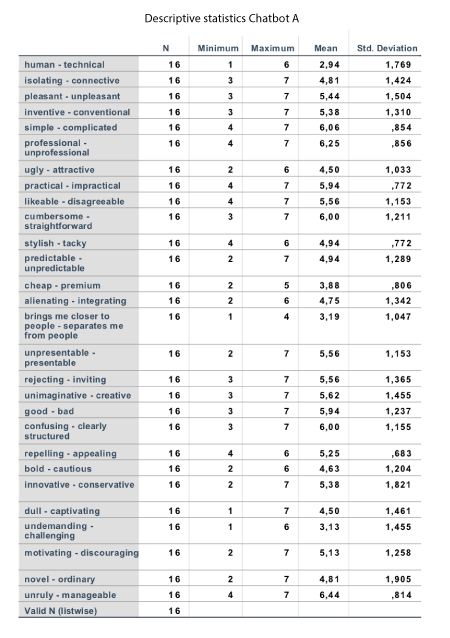
\includegraphics[scale=0.8]{figures/DescriptiveChatbotA.png}
        \caption{Descriptive statistics word pairs Chatbot A}
        \label{fig:deschatA}
    \end{figure}
    
    \begin{figure}[H]
        \centering
        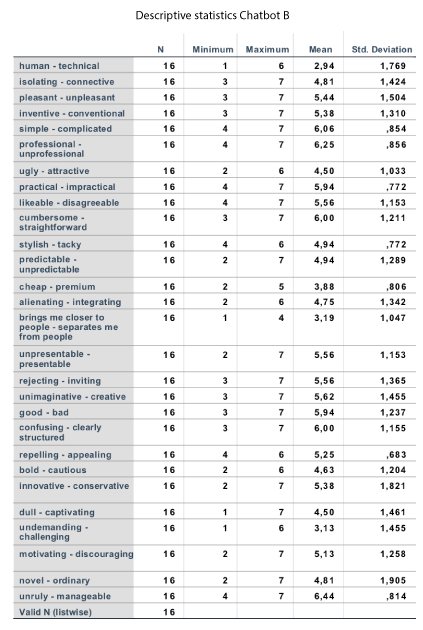
\includegraphics[scale=0.8]{figures/DescriptiveChatbotB.png}
        \caption{Descriptive statistics word pairs Chatbot B}
        \label{fig:deschatB}
    \end{figure}



%\include{inc/timetable}

\end{document}
